%%%%%% USE PDFLATEX !!! %%%%%
%% CMD pdflatex -synctex=1 -shell-escape -interaction=nonstopmode %.tex %%
\documentclass[a4paper, 11pt,twoside=true]{scrartcl}
\usepackage{geometry}
\usepackage[table,xcdraw]{xcolor}
\usepackage{Rapport2}
\usepackage{enumitem}
\usepackage{lipsum}
\usepackage{listings}
\usepackage{enumitem}
\usepackage{minted}

\graphicspath{{./}{./img/}{./fig/}{./image/}{./figure/}{./picture/}
	{./imgs/}{./figs/}{./images/}{./figures/}{./pictures/}}

\setenumerate[1]{itemsep=0pt,partopsep=0pt,parsep=\parskip,topsep=5pt}
\setitemize[1]{itemsep=0pt,partopsep=0pt,parsep=\parskip,topsep=5pt}
\setdescription{itemsep=0pt,partopsep=0pt,parsep=\parskip,topsep=5pt}


\newcommand{\lab}{Report of \textit{Introduction to data science}}
\newcommand{\tit}{My View on Data Science \& Application in COVID-19}
\newcommand{\nom}{NORM}
\newcommand{\superv}{Superviseur}
\newcommand{\depa}{Computer science and technology}
\newcommand{\ID}{222019321102021\\}
\author{Kairui Liu\\}
\newcommand{\names}{Kairui Liu\\}
\automark[section]{section}

\lehead*{%
  \makebox[0pt][r]{
    \colorbox{rahmen}{\makebox[\textwidth][r]{\bfseries\color{white}{\pagemark/\pageref*{LastPage}}\enskip}}\hspace*{1em}}%
  \headmark\hspace*{1em}\headrulefill%
}
\rohead*{%
  \headrulefill\hspace*{1em}\headmark%
  \makebox[0pt][l]{%
    \hspace*{1em}\colorbox{rahmen}{\makebox[\textwidth][l]{\enskip\bfseries\color{white}{\pagemark/\pageref*{LastPage}}}}}%
}
\lefoot{\color{darkgray}\small  2020年6月23日}
\rofoot{\color{darkgray}\small  2020年6月23日}
\cefoot{\color{darkgray}\small \itshape \tit\unskip\strut}
\cofoot{\color{darkgray}\small \itshape \qquad \qquad \tit\unskip\strut}
%%%%%%%%%%%%%%not????
\refoot{\color{darkgray}\small 数据科学导论课程报告\unskip\strut}
\lofoot{\color{darkgray}\small 2019 计算机科学与技术 01班\unskip\strut}

\addtokomafont{pagenumber}{\bfseries\color{white}}
\newcommand\headrulefill{\leaders\hrule width 0pt height 3pt depth -2.8pt \hfill}

%\renewcommand\titlepagestyle{empty}

\hfuzz 100pt
\hbadness 10000
\hfuzz 100pt
\hbadness 10000

% Inversion des espaces des marges

\let\tempmargin\oddsidemargin
\let\oddsidemargin\evensidemargin
\let\evensidemargin\tempmargin
\reversemarginpar

\sisetup{detect-weight=true, detect-family=true}

\renewcommand*{\maketitle}{%
\begin{titlepage}
\raggedleft
\includegraphics[scale=0.5]{sect_physique_pant}

\begin{center}
\horrule{0.5pt} \\[0.4cm] \vspace{-1.5ex}\textcolor{darkblue}
	 { \huge \bfseries \lab \\ \vspace{0.4cm} \tit }\\[0.1cm]\horrule{2pt} \vspace{-4ex}
%\horrule{0.5pt} \\[0.4cm] \vspace{-1.5ex}\textcolor{darkblue}
%	 { \huge \bfseries \lab \\ \vspace{0.4cm} \tit }\\[0.1cm]\horrule{2pt} \vspace{-2ex}
\end{center}
\vspace{1cm}
\begin{center}
 \textsc{\LARGE 西南大学\\ \large 计算机与信息科学学院 软件学院 \\ \depa \\ 数据科学导论 \unskip\strut} \vspace{-3ex} \\	
% \textsc{\LARGE Southwest University\\ \large School of computer and information science, school of software \\ \depa\unskip\strut} \vspace{-1.5ex} \\	
\end{center}
\vspace{3cm}
\begin{minipage}[t]{0.5\textwidth}
	\begin{flushleft}
		{\large \textit{年级} \\ 2019\unskip\strut
		}
	\end{flushleft}
\end{minipage}%
%
\begin{minipage}[t]{0.5\textwidth}
	\begin{flushright}
		{\large \textit{学号} \\ \ID\unskip\strut}           
		\vspace*{0.2cm}
	\end{flushright}    
\end{minipage}%

\begin{minipage}[t]{0.5\textwidth}
	\begin{flushleft}
		{\large \textit{班级}\\ 计算机科学与技术 01班	\unskip\strut
		}
	\end{flushleft}
\end{minipage}%
%
\begin{minipage}[t]{0.5\textwidth}
	\begin{flushright}
		{\large \textit{姓名}\\ \names	\unskip\strut}           
		\vspace*{0.5cm}
	\end{flushright}    
\end{minipage}%

\vspace{3.5cm}
\begin{center}
\begin{minipage}[h]{\textwidth}
    \vfill
    \begin{center}
        {\large 授课教师:陈怀东  \\ 2020年6月23日}
    \end{center}    
\end{minipage}%
\end{center}

\end{titlepage}
}
 

\begin{document}

%%%%TITRE

%\newgeometry{left=3.8cm,right=2.5cm,bottom=0cm}
\newgeometry{left=2.8cm,right=2.8cm,bottom=0cm}
%\newgeometry{left=2.5cm,right=3.8cm,bottom=0cm}
\maketitle
\restoregeometry
\section*{Abstract}
\qquad Data science is an emerging discipline that combines statistics, data analysis, machine learning and related methods, and aims to use data to "understand and analyze" actual phenomena. In short: data science is a discipline that makes data useful. In this report, I will start with the data science I understand, try to use the data set, continue the limited analysis of the data and get interesting and reasonable conclusions.

\quad In the first part of the report, I expounded what I think of data science and what is data science. As an emerging discipline, data science contains the knowledge of those disciplines. In the time of big data, how the data science apply in various fields.What are the new technologies in the development of data science, what challenges have scientists and data science encountered as a newly budding discipline, and the future development prospects of data science.

\quad In the second part of the report, I tried to access data.gov and data.govt.nz, tried to find the data sets that I was interested in and validated, and tried to download and analyze them. I downloaded the Foci statistics of cancer deaths in New Zealand from 1948 to 2011and the daily PM2.5 concentration data of New Zealand cities from 2008 to 2017. I imported this data set into R. I used ggplot to perform a very simple data visualization of the data set, but I got Many unexpected results. After that, I discussed the advantages and disadvantages of data opening. Then I discussed the questions of our government in data opening. Finally I compared our government data disclosure platform with the platforms of countries that used data open platforms earlier, and give feasible advice

\quad In the third part of the report, I tried to analyze the global transmission data of COVID-19 on April 19, 2020, and tried to use R clustering and Q clustering combined with principal component analysis to obtain a quantitative definition of the global of disease , And by using the response surface prediction model and an improved SEIR model based on COVID-19 in both statistics and epidemiology, and combining to obtain a quantitative definition of the disease pandemic, a prediction model for the number of asymptomatic infections is obtained. The model has High accuracy

\quad  In the semester of data science, I not only learned how to use the R language tool, but more importantly, I learned how to analyze the existing data scientifically, examine the problems with the eyes of the data scientist, and analyze the problems in life. Problems are combined with mathematical models to optimize our decisions\\
\\
\textbf{keywords:} Data science; R language; Data opening; Cluster analysis; Principal component analysis; Response surface prediction; Modified SEIR model; COVID-19

\newpage
\newgeometry{left=3.8cm,right=2.5cm,bottom=0cm}
\setcounter{page}{1}
\tableofcontents
\newpage
\newcounter{thispage}
\restoregeometry
%%%%%%% Début du document

\section{My Review and Outlook of Data Science}
\subsection*{Abstract}
\addcontentsline{toc}{subsection}{Abstract}
\qquad The $21^{st}$ century has ushered in the age of big data and data economy, data science emerged as a new and important discipline, in which data carries important knowledge, insights, and potential. An appropriate understanding of data and its organisms relies on the new field of data science and its keystone, analytics. Although it is widely debated whether big data is only hype, and data science is still in a very early phase, significant challenges and opportunities are emerging or have been inspired.  In data science, existing approaches need to be combined to turn abundantly available data into value for individuals, organizations, and society. Moreover, new challenges have emerged, not just in terms of size ("Big Data") but also in terms of the questions to be answered. 

\quad This article provides overviews and prospect of the  data science.  Including my opinion of data science, the technology, application, and prospect.\\
\\
\textbf{keywords:} Process Mining; Data Science; Event Data; Data Analytics; Computing; Informatics; data economy; Data industry 

\subsection{What is data science \& what is included in data science}
\qquad The term "data science" has existed for the better part of the last 30 years and was originally used as a substitute for "computer science" in 1960. Approximately 15 years later, the term was used to define the survey of data processing methods used in different applications. In 2001, data science was introduced as an independent discipline. The Harvard Business Review published an article in 2012 describing the role of the data scientist as the "sexiest job of the $21^st$ century."

\quad Data science provides meaningful information based on large amounts of complex data or big data Data science, or data-driven science, combines different fields of work in statistics and computation to interpret data for decision-making purposes.\\
\textbf{Data science includes Data Mining, Big Data and Data Analysis.}

\quad Data Mining is a main branch of Data Science. Data Mining is devoted to overcoming long-standing unresolved problems related to massive data and small data. Data mining is the process of discovering patterns in large data sets involving methods at the intersection of machine learning, statistics, and database systems. Data mining is an interdisciplinary subfield of computer science and statistics with an overall goal to extract information from a data set and transform the information into a comprehensible structure for further use. Aside from the raw analysis step, it also involves database and data management aspects, data pre-processing, model and inference considerations, interestingness metrics, complexity considerations, post-processing of discovered structures and visualization.

\quad Big data is a field that treats ways to analyze, systematically extract information from, or otherwise deal with data sets that are too large or complex to be dealt with by traditional data-processing application software. Data with many cases offer greater statistical power, while data with higher complexity may lead to a higher false discovery rate. Big data challenges include capturing data, data storage, data analysis, search, sharing, transfer, visualization, querying, updating, information privacy and data source. Big data was originally associated with three key concepts: volume, variety, and velocity.

\quad Data analysis is a process of inspecting, cleansing, transforming and modeling data with the goal of discovering useful information, informing conclusions and supporting decision-making. Data analysis has multiple facets and approaches, encompassing diverse techniques under a variety of names, and is used in different business, science, and social science domains. In today's business world, data analysis plays a role in making decisions more scientific and helping businesses operate more effectively.

\subsection{Applications of Data Science}
\qquad With the development of data science, data science has been widely used in more and more fields. Almost all aspects of research require and generate big data. Therefore, data science has its place.

\quad In the report \textit{Where Analytics, Data Science, Machine Learning Were Applied(2019): Trends and Analysis}  CRM/Consumer analytics, health care, banking, finance, and science were the top sectors in 2018. (Statistics of complete application fields of data science are in appendix A)
\begin{enumerate}
\item CRM/Consumer analytics, 18.6\%\\
\item Health care, 17.2\%\\
\item Banking, 17.0\%\\
\item Finance, 16.1\%\\
\item Science, 13.6\%\\
\end{enumerate}
The trend of data science application rate in various aspects is shown in the Figure.\ref{P1F1}

\begin{figure}[h]
	\small
	\centering
	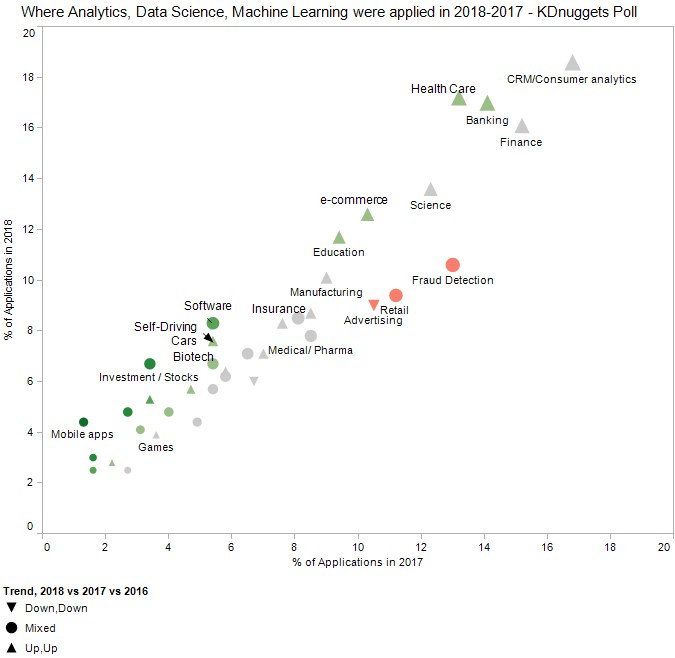
\includegraphics[width=11cm]{P1F1}
	\caption{Where Analytics, Data Science, Machine Learning were applied in 2017, 2018 - KDnuggets Polls} \label{P1F1}
\end{figure}

\quad Data science is very useful in scientific research. Data technology can mine the information and knowledge hidden in massive data to provide a basis for human social and economic activities, thereby improving the operational efficiency of various fields and greatly increasing the intensification of the entire social economy degree. In my country, big data will focus on the following three areas: business intelligence, government decision-making, and public services. For example: business intelligence technology, government decision-making technology, telecommunications data information processing and mining technology, power grid data information processing and mining technology, meteorological information analysis technology, environmental monitoring technology, police cloud application system (road monitoring, video monitoring, network monitoring, Public security information systems such as intelligent transportation, anti-telecom fraud, command and dispatch), large-scale gene sequence analysis and comparison technology, Web information mining technology, multimedia data parallel processing technology, film and television production rendering technology, cloud computing and massive in other industries Data processing application technology, etc..

\subsection{New Technologies of Data Science}
\qquad Data Science has become an integral part of those transformations. With Data Science, organizations no longer have to make their important decisions based on hunches, best-guesses, or small surveys. Instead, they’re analyzing large amounts of real data to base their decisions on real, data-driven facts. That’s really what Data Science is all about — creating value through data.\\
\textbf{1. Automated Data Science}

\quad Even in today’s digital age, Data Science still requires a lot of manual work. Storing data, cleaning data, visualizing and exploring data, and finally, modeling data to get some actual results. Nearly every step of the Data Science pipeline has been or is in the process of becoming automated. 

\quad In general, companies are investing heavily in building and buying tools and services for automated Data Science. Anything to make the process cheaper and easier. At the same time, this automation also caters to smaller and less technical organizations that can leverage these tools and services to have access to Data Science without building out their own team.\\
\textbf{2. Super-sized Data Science in the Cloud}

\quad Over the years that Data Science has grown from a niche to its own full-on field, the data available for analysis has also exploded in size. Organizations are collecting and storing more data than ever before.

\quad The volume of data that a typical Fortune 500 company might need to analyze has gone far past what a personal computer can handle. A decent PC might have something like 64GB of RAM with an 8 core CPU and 4TB of storage. That works just fine for personal projects, but not so well when you work for a global company such as a bank or retailer who has data covering millions of customers.\\
\textbf{3. Natural Language Processing}

\quad Natural Language Processing (NLP) has made its way firmly into Data Science after huge breakthroughs in Deep Learning research.

\quad Huge advancements in NLP through Deep Learning are fueling the full-on integration of NLP into our regular Data Analysis. Neural Networks can now extract information from large bodies of text incredibly quickly. They’re able to classify text into different categories, determine sentiment about a text, and perform analysis on the similarity of text data. In the end, all of that information can be stored in a single feature vector of numbers.

\quad As a result, NLP becomes a powerful tool in Data Science. Huge datastores of text, not just one-word answers but full-on paragraphs, can be transformed into numerical data for standard analysis. 

\subsection{The Challenges of Data Science}
\qquad Data is a lucrative field to pursue, and there’s plenty of demand for people with related skills. However, no career is without its challenges, and data science is not an exception. Data science is about finding useful insights and putting them to use. Data science, however, doesn’t occur in a vacuum. When pursuing their analytics goals, data professionals can be confronted by different types of challenges that hinder their progress. In this section, I want to talk about the Challenges of Data Science.

\quad In the report \textit{Top 10 Challenges to Practicing Data Science at Work},the survey asked respondents, "At work, which barriers or challenges have you faced this past year?." Results appear in Figure.\ref{P1F2} and show that the top 10 challenges were:\\
\begin{enumerate}
\item Dirty data (36\%) \\
\item Lack of data science talent (30\%) \\
\item Company politics (27\%) \\
\item Lack of clear question (22\%) \\
\item Data inaccessible (22\%) \\
\item Results not used by decision makers (18\%) \\
\item Explaining data science to others (16\%) \\
\item Privacy issues (14\%) \\
\item Lack of domain expertise (14\%) \\
\item Organization small and cannot afford data science team (13\%)\\
\end{enumerate}

\begin{figure}[h]
	\small
	\centering
	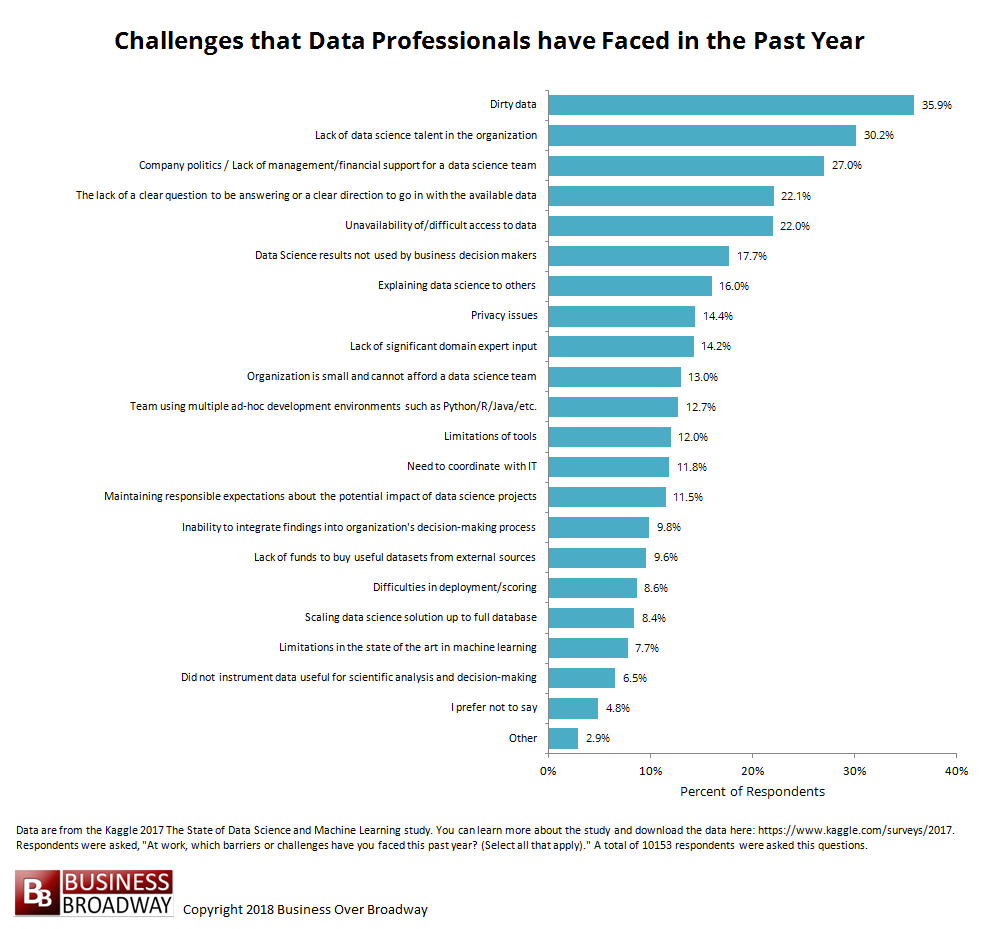
\includegraphics[width=13cm]{P1F2}
	\caption{Challenges data scientist meet} \label{P1F2}
\end{figure}

\quad Results revealed that, on average, data professionals reported experiencing three (median) challenges in the previous year. The number of challenges experienced varied significantly across job title. Data professionals who self-identified as a Data Scientist or Predictive Modeler reported using four platforms. Data pros who self-identified as a Programmer reported only one challenge.

\quad Data professionals experience challenges in their data science and machine learning pursuits. Data professionals experience about three challenges in a year. The most common data science and machine learning challenges included dirty data, lack of data science talent, lack of management support and lack of clear direction/question.
	
\subsection{outlook for data scientists and data science}
\qquad Data science is an interdisciplinary area of scientific processes, methods, systems, and algorithms to obtain knowledge or awareness of data in an array of forms. The field combines data analysis, statistics, and machine learning and their associated methods to gain an understanding and evaluate data. It uses theories and procedures drawn from a variety of fields and data scientists are analytical data experts who possess technical abilities to solve multifaceted problems. Data scientists take a large amount of complicated data points, both structured and unstructured, and use their abilities to clean and organize them. They sold business challenges by applying their analytic skills, including industry knowledge, contextual understanding, and doubt of current assumptions. Individuals interested in working in the data science field often wonder about the job outlook for data scientists.

\quad As stated by the United States of Labor Statistics, the employment of all computer and information research scientists is expected to rise 19 percent by the year 2026, which is deemed much faster than the average for all professions. About 5,400 new jobs are projected over the decade. As demand for new and improve technology increases in the data science field, the demand for qualified data scientists will rise. The rapid growth in data collection will result in a heightened need for data-mining services.

\quad Data Science is an ever growing field and is expected to grow in demand in the foreseeable future. Some of the key changes are listed below.

\quad 1. \textbf{Data}: With the radical increase of generation of data, the performance of the predictive algorithms is going to improve over time as more structured data is available to draw inference upon. This phenomenon is fueled by the growth of Social Media and IoT based devices, which generate a lot more structured data.

\quad 2. \textbf{Algorithms}: Machine Learning algorithms like Genetic Algorithms and Reinforcement Learning algorithms are expected to improve over time causing more intelligent systems.

\quad 3. \textbf{Distributed Computing}: With the advancements of blockchain technology, TPU (Tensor Processing Unit) development and faster GPU (Graphics Processing Unit) available in the cloud, Data Science sees a future where more powerful computational hardware aids the algorithms of increasing complexity.

\quad More Data and improved Algorithms and Hardware together are expected to bring significant improvements in the field of Data Science in the near future.

\subsection{Summary}
\qquad Data Science is a hyped up complex field of study. For the most part, the choose is true and it delivers solutions to problems as promised. Some fields of data science have even started to outperform humans and that trend is expected to increase in the near future. You can take up Data Science training to enhance your career.

\quad Data Science defines the bleeding edge of technology at present and promises further technological advancements in the near future. It is also one of the most in-demand and high paying jobs in the industry. Hence, there is no better time to be a Data Scientist than now!

\begin{thebibliography}{99}
	\addcontentsline{toc}{subsection}{Reference}
	\bibitem{1}Cao, L. (2017). Data Science: A Comprehensive Overview. ACM Computing Surveys, 50(3).
	\bibitem{2}van der Aalst W. (2016) Data Science in Action. In: Process Mining. Springer, Berlin, Heidelberg
	\bibitem{3}Banton, C. (2019). Inside Data Science and Its Applications. Retrieved 8 June 2020, from https://www.investopedia.com/terms/d/data-science.asp
	\bibitem{4}Data mining. (2020). Retrieved 8 June 2020, from https://en.wikipedia.org/wiki/Data\_mining
	\bibitem{5}Data analysis. (2020). Retrieved 8 June 2020, from https://en.wikipedia.org/wiki/D
	ata\_analysis
	\bibitem{6}Mayo, M. (2019). Where Analytics, Data Science, Machine Learning Were Applied:
	Trends and Analysis - KDnuggets. Retrieved 8 June 2020, from https://www.kdnuggets.com
	/2019/03/poll-analytics-data-science-ml-applied-2018.html
	\bibitem{7}How is the job outlook for data scientists?. (2020). Retrieved 8 June 2020, from https://www.datasciencedegreeprograms.net/faq/job-outlook-data-scientists/
	\bibitem{8}Hayes, B. (2020). Top 10 Challenges to Practicing Data Science at Work. Retrieved 8 June 2020, from https://businessoverbroadway.com/2018/03/18/top-10-challenges-to-practicing-data-science-at-work
	\bibitem{9}Seif, G. (2020). The 4 Hottest Trends in Data Science for 2020 - KDnuggets. Retrieved 8 June 2020, from https://www.kdnuggets.com/2019/12/4-hottest-trends-data-science-2020.html
\end{thebibliography}

\newpage
\subsection*{Appendix}
\addcontentsline{toc}{subsection}{Appendix}
\subsubsection*{Appendix A: Industry applied data science, data analysis}
\begin{table}[H]
	\begin{tabular}{
			>{\columncolor[HTML]{FFFFFF}}l 
			>{\columncolor[HTML]{FFFFFF}}l 
			>{\columncolor[HTML]{FFFFFF}}l 
			>{\columncolor[HTML]{FFFFFF}}l }
		\hline
		{\color[HTML]{000000} \textbf{Fields}}                       & {\color[HTML]{000000} \textbf{2018}} & {\color[HTML]{000000} \textbf{2017}} & {\color[HTML]{000000} \textbf{2016}} \\ \hline
		{\color[HTML]{000000} CRM/Consumer analytics (81)}           & {\color[HTML]{000000} 18.60}         & {\color[HTML]{000000} 16.80}         & {\color[HTML]{000000} 16.30}         \\
		{\color[HTML]{000000} Health care (75)}                      & {\color[HTML]{000000} 17.20}         & {\color[HTML]{000000} 13.20}         & {\color[HTML]{000000} 12.00}         \\
		{\color[HTML]{000000} Banking (74)}                          & {\color[HTML]{000000} 17.00}         & {\color[HTML]{000000} 14.10}         & {\color[HTML]{000000} 13.40}         \\
		{\color[HTML]{000000} Finance (70)}                          & {\color[HTML]{000000} 16.10}         & {\color[HTML]{000000} 15.20}         & {\color[HTML]{000000} 15.00}         \\
		{\color[HTML]{000000} Science (59)}                          & {\color[HTML]{000000} 13.60}         & {\color[HTML]{000000} 12.30}         & {\color[HTML]{000000} 12.00}         \\
		{\color[HTML]{000000} E-commerce (55)}                       & {\color[HTML]{000000} 12.60}         & {\color[HTML]{000000} 10.30}         & {\color[HTML]{000000} 8.90}          \\
		{\color[HTML]{000000} Education (51)}                        & {\color[HTML]{000000} 11.70}         & {\color[HTML]{000000} 9.40}          & {\color[HTML]{000000} 7.10}          \\
		{\color[HTML]{000000} Fraud Detection (46)}                  & {\color[HTML]{000000} 10.60}         & {\color[HTML]{000000} 13.00}         & {\color[HTML]{000000} 11.10}         \\
		{\color[HTML]{000000} Manufacturing (44)}                    & {\color[HTML]{000000} 10.10}         & {\color[HTML]{000000} 9.00}          & {\color[HTML]{000000} 5.60}          \\
		{\color[HTML]{000000} Retail (41)}                           & {\color[HTML]{000000} 9.40}          & {\color[HTML]{000000} 11.20}         & {\color[HTML]{000000} 10.30}         \\
		{\color[HTML]{000000} Advertising (39)}                      & {\color[HTML]{000000} 9.00}          & {\color[HTML]{000000} 10.50}         & {\color[HTML]{000000} 12.00}         \\
		{\color[HTML]{000000} Supply Chain (38)}                     & {\color[HTML]{000000} 8.70}          & {\color[HTML]{000000} 8.50}          & {\color[HTML]{000000} 6.50}          \\
		{\color[HTML]{000000} Insurance (37)}                        & {\color[HTML]{000000} 8.50}          & {\color[HTML]{000000} 8.10}          & {\color[HTML]{000000} 9.20}          \\
		{\color[HTML]{000000} Software (36)}                         & {\color[HTML]{000000} 8.30}          & {\color[HTML]{000000} 5.40}          & {\color[HTML]{000000} 7.20}          \\
		{\color[HTML]{000000} IT / Network Infrastructure (36)}      & {\color[HTML]{000000} 8.30}          & {\color[HTML]{000000} 7.60}          & {\color[HTML]{000000} 7.20}          \\
		{\color[HTML]{000000} Other (34)}                            & {\color[HTML]{000000} 7.80}          & {\color[HTML]{000000} 8.10}          & {\color[HTML]{000000} 6.30}          \\
		{\color[HTML]{000000} Medical/ Pharma (34)}                  & {\color[HTML]{000000} 7.80}          & {\color[HTML]{000000} 8.50}          & {\color[HTML]{000000} 6.50}          \\
		{\color[HTML]{000000} Automotive/ Self-Driving Cars (33)}    & {\color[HTML]{000000} 7.60}          & {\color[HTML]{000000} 5.40}          & {\color[HTML]{000000} 4.50}          \\
		{\color[HTML]{000000} Oil / Gas / Energy (31)}               & {\color[HTML]{000000} 7.10}          & {\color[HTML]{000000} 6.50}          & {\color[HTML]{000000} 7.10}          \\
		{\color[HTML]{000000} Credit Scoring (31)}                   & {\color[HTML]{000000} 7.10}          & {\color[HTML]{000000} 7.00}          & {\color[HTML]{000000} 6.90}          \\
		{\color[HTML]{000000} Investment / Stocks (29)}              & {\color[HTML]{000000} 6.70}          & {\color[HTML]{000000} 3.40}          & {\color[HTML]{000000} 6.20}          \\
		{\color[HTML]{000000} Biotech/Genomics (29)}                 & {\color[HTML]{000000} 6.70}          & {\color[HTML]{000000} 5.40}          & {\color[HTML]{000000} 5.80}          \\
		{\color[HTML]{000000} Government / Military (28)}            & {\color[HTML]{000000} 6.40}          & {\color[HTML]{000000} 5.80}          & {\color[HTML]{000000} 5.60}          \\
		{\color[HTML]{000000} Telecom / Cable (27)}                  & {\color[HTML]{000000} 6.20}          & {\color[HTML]{000000} 5.80}          & {\color[HTML]{000000} 8.30}          \\
		{\color[HTML]{000000} Social Media / Social Networks (26)}   & {\color[HTML]{000000} 6.00}          & {\color[HTML]{000000} 6.70}          & {\color[HTML]{000000} 8.30}          \\
		{\color[HTML]{000000} HR/workforce analytics (25)}           & {\color[HTML]{000000} 5.70}          & {\color[HTML]{000000} 4.70}          & {\color[HTML]{000000} 3.60}          \\
		{\color[HTML]{000000} Search / Web content mining (25)}      & {\color[HTML]{000000} 5.70}          & {\color[HTML]{000000} 5.40}          & {\color[HTML]{000000} 5.40}          \\
		{\color[HTML]{000000} Agriculture (23)}                      & {\color[HTML]{000000} 5.30}          & {\color[HTML]{000000} 3.40}          & {\color[HTML]{000000} 3.30}          \\
		{\color[HTML]{000000} Entertainment/ Music/ TV/ Movies (21)} & {\color[HTML]{000000} 4.80}          & {\color[HTML]{000000} 2.70}          & {\color[HTML]{000000} 4.00}          \\
		{\color[HTML]{000000} Travel / Hospitality (21)}             & {\color[HTML]{000000} 4.80}          & {\color[HTML]{000000} 4.00}          & {\color[HTML]{000000} 4.00}          \\
		{\color[HTML]{000000} Mobile apps (19)}                      & {\color[HTML]{000000} 4.40}          & {\color[HTML]{000000} 1.30}          & {\color[HTML]{000000} 3.30}          \\
		{\color[HTML]{000000} Direct Marketing/ Fundraising (19)}    & {\color[HTML]{000000} 4.40}          & {\color[HTML]{000000} 4.90}          & {\color[HTML]{000000} 4.30}          \\
		{\color[HTML]{000000} Mining (18)}                           & {\color[HTML]{000000} 4.10}          & {\color[HTML]{000000} 3.10}          & {\color[HTML]{000000} 4.20}          \\
		{\color[HTML]{000000} Games (17)}                            & {\color[HTML]{000000} 3.90}          & {\color[HTML]{000000} 3.60}          & {\color[HTML]{000000} 2.90}          \\
		{\color[HTML]{000000} Security / Anti-terrorism (13)}        & {\color[HTML]{000000} 3.00}          & {\color[HTML]{000000} 1.60}          & {\color[HTML]{000000} 2.70}          \\
		{\color[HTML]{000000} Junk email / Anti-spam (12)}           & {\color[HTML]{000000} 2.80}          & {\color[HTML]{000000} 2.20}          & {\color[HTML]{000000} 1.10}          \\
		{\color[HTML]{000000} Social Policy / Survey analysis (11)}  & {\color[HTML]{000000} 2.50}          & {\color[HTML]{000000} 1.60}          & {\color[HTML]{000000} 1.80}          \\
		{\color[HTML]{000000} Social Good / Non-profit (11)}         & {\color[HTML]{000000} 2.50}          & {\color[HTML]{000000} 2.70}          & {\color[HTML]{000000} 2.00}          \\ \hline
	\end{tabular}
\end{table}
\newpage
\subsubsection*{Appendix B: The 40 data science techniques}
\begin{table}[h]
	\begin{tabular}{ll}
		Linear Regression                            & Decision Trees                       \\
		Logistic Regression                          & Random Numbers                       \\
		Jackknife Regression                         & Monte-Carlo Simulation               \\
		Density Estimation                           & Bayesian Statistics                  \\
		Confidence Interval                          & Naive Bayes                          \\
		Test of Hypotheses                           & Principal Component Analysis - (PCA) \\
		Pattern Recognition                          & Ensembles                            \\
		Clustering - (aka Unsupervised Learning)     & Neural Networks                      \\
		Supervised Learning                          & Support Vector Machine - (SVM)       \\
		Time Series                                  & Nearest Neighbors - (k-NN)           \\
		Feature Selection - (aka Variable Reduction) & Linkage Analysis                     \\
		Indexation / Cataloguing                     & Association Rules                    \\
		(Geo-) Spatial Modeling                      & Scoring Engine                       \\
		Recommendation Engine                        & Segmentation                         \\
		Search Engine                                & Predictive Modeling                  \\
		Attribution Modeling                         & Graphs                               \\
		Collaborative Filtering                      & Deep Learning                        \\
		Rule System                                  & Game Theory                          \\
		Feature Selection - (aka Variable Reduction) & Association Rules                    \\
		Indexation / Cataloguing                     & Survival Analysis                    \\
		(Geo-) Spatial Modeling                      & Arbitrage                            \\
		Recommendation Engine                        & Lift Modeling                        \\
		Search Engine                                & Yield Optimization                   \\
		Attribution Modeling                         & Cross-Validation                     \\
		Collaborative Filtering                      & Model Fitting                        \\
		Rule System                                  & Relevancy Algorithm                  \\
		Linkage Analysis                             & Experimental Design                 
	\end{tabular}
\end{table}

\newpage
\section{Introduction to public data sets and my opinion on data disclosure}
\subsection{Introduction to Government Data}
\qquad In this section, this paper will introduce two pieces of data set of New Zealand governments.

\quad All data in this section comes from New Zealand government data.govt.nz and follows the CC 4.0 BY-SA copyright agreement
\subsubsection{Introduction to the first dataset: PM2.5 concentrations, 2008–17}
\qquad PM2.5 is made up of solid and liquid particles in the air with a diameter of less than 2.5 micrometers. In New Zealand, most PM2.5 in the air results from combustion (burning wood for home heating, motor-vehicle exhaust), and to a lesser extent, particles formed from reactions in the atmosphere (secondary PM) and naturally occurring sea salt. Short- and long-term exposure to PM2.5, even at low levels, is linked to respiratory and cardiovascular disease, and increased risk of premature death, especially in vulnerable people (the young, the elderly, and people with respiratory illness). The dataset record the concentrations of PM2.5 by day from 2008 to 2017

\quad This data set contains the data of the city to be tested, the date of the test, the test institution, the test method, the PM2.5 value, and whether all data for the current year are completely recorded. Record created February 2, 2020, Last Updated June 2, 2020.

\quad I imported the data set into R and tried to view the shape and structure of the data set. Fortunately, the data of this data set almost did not need to be cleaned, and the data was very clean. We can easily see the structure and characteristics of the data through ggplot. The data has a lot of very interesting features, these features surprised me very much, the results are very interesting

\noindent \textbf{1. First, we import the data into R}
\begin{minted}%
	[encoding=utf8,
	linenos,
	frame=single,
	rulecolor=purple!50!black,
	texcl=true,
	highlightcolor=green!40,
	]{R}
library(tidyverse)
library(lubridate)
setwd("C:/Users/tclkr/Desktop/D1")
pm25<-read_csv("./pm25.csv")
Sys.setlocale("LC_TIME", "English")
\end{minted}
\textbf{2. At first, I just want to sort and summarize the daily PM2.5 data to check the change rule of PM2.5 concentration}
\begin{minted}%
[encoding=utf8,
linenos,
frame=single,
rulecolor=purple!50!black,
texcl=true,
highlightcolor=green!40,
]{R}
byy<-pm25%>%
  select(site,date,pm2_5)%>%
  group_by(date)%>%
  summarize(val=mean(pm2_5,na.rm=TRUE))

ggplot(data=byy)+
  geom_point(mapping = aes(x=date,y=val),size=0.35)+
  labs(x="Date",y="Concentration")
\end{minted}
\begin{figure}[h]
	\small
	\centering
	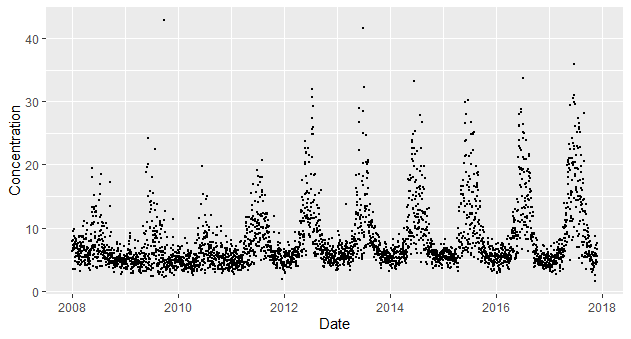
\includegraphics[width=13cm]{P2F1}
	\caption{Historical change chart of PM2.5 concentration} \label{P2F1}
\end{figure}
In the Figure.\ref{P2F1}, PM2.5 concentration is rising, but it will rise and fall once a year, which arouses my research interest\\
\textbf{3. I want to count the average concentration of PM2.5 in each month}
\begin{minted}%
[encoding=utf8,
linenos,
frame=single,
rulecolor=purple!50!black,
texcl=true,
highlightcolor=green!40,
breaklines=true,
]{R}
bymon_day<-pm25%>%
  select(date,pm2_5)%>%
  mutate(date_in_year=make_date(2020,month(date),day(date)))%>%
  group_by(date_in_year)%>%
  summarize(mean_value=mean(pm2_5,na.rm=TRUE))


ggplot(data=bymon_day,mapping = aes(x=date_in_year,y=mean_value))+
  geom_point(alpha=0.3)+
  geom_smooth(method="loess")+
  scale_x_date(date_breaks = "1 month",date_minor_breaks = "1 month", date_labels = "%b")+
  labs(x="Date",y="Concentration")

\end{minted}
\begin{figure}[h]
	\small
	\centering
	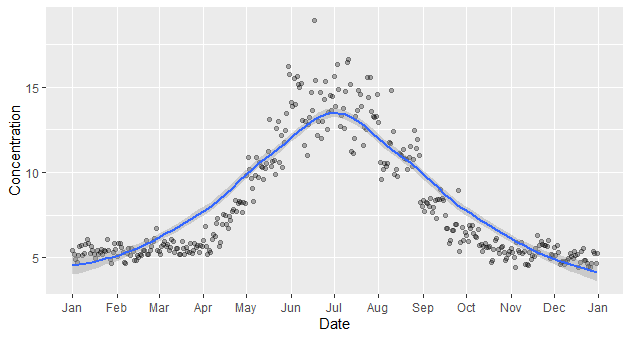
\includegraphics[width=13cm]{P2F2}
	\caption{Monthly change chart of PM2.5 concentration} \label{P2F2}
\end{figure}
As I expected, in Figure.\ref{P2F2}the PM2.5 concentration first increased and then decreased in a year, but what I didn’t think was that the regression curve was so regular, and the confidence interval was so small, which made me want to study its normality through the QQ chart(Figure.\ref{P2F3})to distribution correlation\\
\begin{minted}%
[encoding=utf8,
linenos,
frame=single,
rulecolor=purple!50!black,
texcl=true,
highlightcolor=green!40,
]{R}
ggplot()+
  qqnorm(bymon_day$mean_value)
\end{minted}
\begin{figure}[h]
	\small
	\centering
	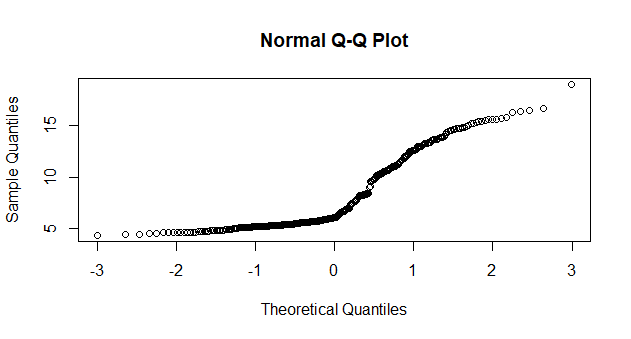
\includegraphics[width=13cm]{P2F3}
	\caption{The QQ chart of the monthly mean change chart of PM2.5 concentration} \label{P2F3}
\end{figure}
\textbf{4.Then I checked the PM2.5 concentration change between each year(Figure.\ref{P2F4})}
\begin{minted}%
[encoding=utf8,
linenos,
frame=single,
rulecolor=purple!50!black,
texcl=true,
highlightcolor=green!40,
]{R}
byyear<-pm25%>%
  select(site,date,pm2_5)%>%
  mutate(years=year(date))%>%
  group_by(years)%>%
  summarize(val=mean(pm2_5),na.rm=TRUE)

ggplot(data=byyear,aes(x=years,y=val))+
  geom_line()+
  geom_point()+
  labs(x="Date",y="Concentration")
\end{minted}
\begin{figure}[h]
	\small
	\centering
	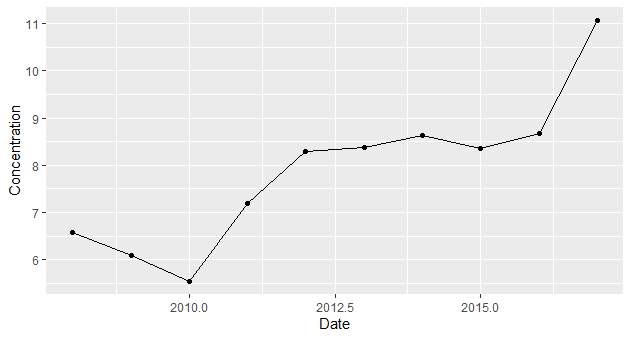
\includegraphics[width=12cm]{P2F4}
	\caption{Diagram of annual change of PM2.5 concentration} \label{P2F4}
\end{figure}
It is a pity that I did not find why the concentration of PM2.5 will drop sharply between 2008 and 2010\\
\textbf{5. Finally, I looked at the average data for each city}\\
\begin{minted}%
[encoding=utf8,
linenos,
frame=single,
rulecolor=purple!50!black,
texcl=true,
highlightcolor=green!40,
breaklines=true,
]{R}
library(maps)
library(mapdata)
library(maptools)
library(rgdal)

bycty<-pm25%>%
  select(site,date,pm2_5)%>%
  group_by(site)%>%
  summarize(val=mean(pm2_5),na.rm=TRUE)
map<-readOGR("./NZL_adm2.shp")
map1 <- fortify(map)
map1 <- as_tibble(map1)
map1 <- filter(map1,long>50)
ggplot()+
  geom_map(mapping = aes(x=map1$long,y=map1$lat))

summary(map1)
\end{minted}

\subsubsection{Introduction to the second dataset: Cancer: Historical summary 1948-2011}
\qquad This data set records a summary of cancer site records and death data from 1948 to 2011. The data was created on May 21, 2018. Sites include: lips, mouth and pharynx, esophagus, stomach, large intestine, liver and intrahepatic bile duct, pancreas, lung, melanoma, breast, cervix, uterus, ovary, vulva, kidney, bladder, brain, thyroid, Hodgkin Lymphoma, non-Hodgkin's lymphoma, myeloma, leukemia. The number of deaths and ASR values are recorded

\quad We should do more work to find out the relationship between them. For example, you can find the relationship between time and cancer types, the proportion of cancer types, and so on.
\subsection{Advantages of Open Data}
\qquad Open data is valuable information that is both free and easily accessible to anyone, without limitations or restrictions. Governments are particularly interested in fostering this new strategy for connecting with their residents, a movement which has become known as open government. Many government bodies have begun to recognize the benefits of conducting more open and transparent operations. Information ranging from legislation, policies, and practices to government performance are being made available to the public through a single source.\\
\textbf{1. Increases transparency and accountability}

\quad The trend towards open data means that members of the public can stay connected, informed, and up to date with the day-to-day operations of their local government. The public nature of this information holds governments accountable to the results they produce. Residents have the ability to see exactly what their government has achieved, and how much more needs to be done. Failure to attain certain results or meet a particular milestone or goal will be publicized and up for public scrutiny. Conversely, achieving or exceeding goals will help to establish a greater and more trusting relationship with local residents.\\
\textbf{2. Develops trust, credibility and reputation}

\quad The transparent nature of publicly accessible data exposes a side of an organization which is quite often kept under wraps. This sort of openness and vulnerability is comparable to sharing aspects of your personal life with another person. There is a considerable amount of trust and respect that comes with an open and honest conversation, and the result is quite often a closer and more dependent relationship between the two parties. In the same way, open government data helps to establish trust and credibility with citizens. Open data can give residents peace of mind that their local government is continually working to deliver on promises and making decisions in the community’s best interests.\\
\textbf{3. Promotes progress and innovation}

\quad The value of key performance data has few bounds when set loose in the public sphere. Open data provides new opportunities for commercial applications, improves time-to-market for businesses, and can form the foundation for new technological innovation and economic growth. Third parties without the resources to gather this data for themselves will be able to re-purpose it and utilize the information to develop new applications and services. Information provided in this way is also significant for academic, public-sector, and industry-based research communities. Open data vastly increases the value of information and allows it to travel and be utilized to its full potential.\\
\textbf{4.  Encourages public education and community engagement}

\quad What better way to educate the community on progress and performance of the city than to have all the information displayed in a clear and user-friendly display? Open government data enables you to proactively answer those frequently asked questions by making the information freely accessible. Information can be made available as quickly as it is gathered, which means that the public can become involved and offer valuable feedback from throughout the entire process. Access to meaningful data aids in unifying a community and empowering them to help shape the direction for the future.\\
\textbf{5. Citizen Participation and Activism}

\quad Citizens are expected to participate in the functioning of a democracy but they are hardly able to do so due to the lack of access to information. Open data can foster citizen participate in.

\subsection{Disadvantages of Open Data}
\textbf{1. Risk of violating legislation by opening data}
\quad Many datasets are and cannot be released for legal or other reasons. Examples of datasets that cannot be made available to the public are datasets which contain privacy identifying variables, sensitive variables and datasets which have been created by multiple organizations which have different levels of security, different policies and have to comply with different laws. Publishing those kind of data would lead to undesirable situations, as this would violate the law and may harm the reputation of the organization that provides these data. \\
\textbf{2. Difficulties with data ownership}

\quad In one of the interviews it was stated that governmental organizations also maintain data of other organizations. These data are not possessed by the governmental organization and, therefore, they cannot be published. Furthermore, when other organizations have contributed to the creation of the data, these data cannot be published. the impact of 'borrowed data’ is high. Much research that we conduct is based on borrowed data. This mainly concerned borrowed data from other governmental organizations. The main reason mentioned for not publishing data that are borrowed or created together with another organization is that the organization does not want to risk reputation damage, as stated by one employee: "one wants to open data but not to stake everything".\\
\textbf{3. Privacy can be violated unintentionally}

\quad Much effort is put on removing privacy sensitive variables from datasets so that they can be opened. One might then think that privacy is guaranteed. Nevertheless by combining data with other sources it might still be possible to track the identity of an individual person, especially when open data are combined with social media data. Guidelines about privacy sensitivity partly help to identify which data cannot be published, but much interpretation effort by the data provider is still required, and combining data could still lead to identifying a person’s identity. \\
\textbf{4. Misinterpretation and misuse}

\quad Very complex data were not made available to the public, because the risk of misinterpretation and misuse was high for these datasets. Moreover, in one of the organizations it was found that some datasets were simply too poorly documented to be able to interpret the data correctly. Data that are made available as open data are freely available to anyone. This also means that people with limited knowledge about how to interpret open data can use them. This might result in incorrect conclusions about the results of an analysis of the data. Some people may even intend to misuse the data to damage the reputation of the data provider. 

\subsection{Advice to Governments On Open Data}
\textbf{1. Government should improve platform services}

\quad When I was studying the \textit{introduction to data science}, I tried to download data from many Chinese government data open platforms, but many of the data request functions of many platforms failed to respond in a timely and effective manner. There are many platforms whose messages have not been answered in time, and the builders of the platform should respond to the user's problems and problems in the process of using the user's feedback and needs in a timely manner, or solve the user's problems if they are not satisfied with the platform. The user's data needs should be promptly responded to, and if the data cannot be provided, the reasons for confidentiality must also be explained.\\
\textbf{2. Open platform should enhance interaction with users}

\quad The interactive communication function of our government data open platform needs to be available after registration. Some platforms require real-name system and ID card registration, which raises the threshold for communication between users and the platform and reduces the requirements for message interaction.\\
\textbf{3. Government should encourage data development and utilization}

\quad At present, thousands of applications and software tools and hundreds of mobile phone plug-ins have been uploaded to the US government data open platform (data.gov). More than one-third of these applications are developed by private programmers and non-profit organizations. Although China's government data open platform has also launched innovative APP activities, the participation of the public is low, and it is not possible to mobilize the interest in participation. There are many open data that cannot meet the data needs of the public to participate in innovative APPs. On some platforms , The submission of APP applications is limited to approved enterprise users, and the audience is relatively narrow, greatly damaging the user's enthusiasm and creativity. Therefore, Chinese government data open platform should first improve the platform's own data quality, followed by more activities, Some rewards can be provided appropriately to stimulate satisfying interest in participation.

\newpage
\begin{thebibliography}{99}
	\addcontentsline{toc}{subsection}{Reference}
	\bibitem{1}Cancer: Historical summary 1948-2011 - data.govt.nz - discover and use data. (2018). Retrieved 31 December 1921, from https://catalogue.data.govt.nz/dataset/cancer-historical-summary-1948-2011
	\bibitem{1}PM2.5 concentrations, 2008–17 - data.govt.nz - discover and use data. (2020). Retrieved 9 June 2020, from https://catalogue.data.govt.nz/dataset/pm2-5-concentrations-200817
	\bibitem{3}Zhang, J. (2018). Research on the development status and countermeasures of Chinese government data opening platform. Heilongjiang: Heilongjiang University.
	\bibitem{4}Wang, L. (2017). Research on government Data Opening from the perspective of holistic governance. Wuhan: Central China Normal University.
	\bibitem{5}Starting an Open Data Initiative. (2019). Retrieved 9 June 2020, from http://opendatatoolkit.worldbank.org/en/starting.html
	\bibitem{6}6 Major Benefits of Open Data – ProWebScraper. Retrieved 9 June 2020, from https://prowebscraper.com/blog/6-major-benefits-of-open-data/
	\bibitem{7}Ong, C. (2016). 5 Benefits of Open Government Data | Envisio. Retrieved 9 June 2020, from https://envisio.com/blog/5-benefits-of-open-government-data/
	\bibitem{8}Pros and Cons of Open Data. (2018). Retrieved 9 June 2020, from https://thesciencefactor.wordpress.com/2018/03/31/pros-and-cons-of-open-data-wcri2017/
	\bibitem{9}Zuiderwijk, A., \& Janssen, M. (2014). The negative effects of open government data - investigating the dark side of open data. digital government research.
\end{thebibliography}

\newpage
\newgeometry{left=3.8cm,right=2.5cm,bottom=0cm}
\section{Quantitative epidemic grading and prediction models for asymptomatic in COVID-19}
\subsection*{Abstract}
\addcontentsline{toc}{subsection}{Abstract}
\textrm{\textbf{\textit{Human hymns are hymns of courage! Human splendor is splendid of courage!}}}
\begin{flushright}\textrm{\textbf{\textit{—— JoJo's Bizarre Adventure}}}\end{flushright}
\qquad As of the writing of the abstract (June 11, 2020), COVID-19 has caused 7221717 infections, of which 411818 deaths. China has made huge sacrifices in the fight against the pneumonia epidemic. At the same time, its active strategy has enabled the rapid spread of pneumonia to be controlled. China’s behavior has been highly appreciated by the WHO. At this time, we have achieved the resumption of production in most industries. The situation in other countries is not optimistic. For example, the development of the US epidemic is very puzzling. The remarks of the US government are puzzling. The government tells people not to wear masks and has withdrawn from the WHO after criticizing each other many times. The US government once believed that WHO’s proposal that the COVID-19 epidemic entered the stage of a global pandemic would cause unnecessary panic on the grounds that although SARS affected 26 countries, it was still not considered a pandemic and MERS was not considered a pandemic. Epidemic. The reason for this controversy is that WHO does not have strict quantitative standards for whether the disease meets the global pandemic, nor does it define a threshold for the number of cases or deaths.

\quad Asymptomatic infected persons are factors that make it difficult to prevent and control the epidemic. Asymptomatic infected persons are infectious and not easy to detect. In the process of resuming labor and resuming labor in China, asymptomatic infections were found in many areas, which seems to have become a new source of infection. On the Internet, we can find many predictions of the development of the COVID-19 epidemic, but it is difficult to obtain data on the number of asymptomatic patients.

\quad Based on the above two points, I obtained the quantitative standard of pandemic disease through the spread data of COVID-19 in various countries and combined with the spread data of H1N1, SARS, MERS.Finally, a prediction model for the number of asymptomatic infections is obtained.

\quad In defining the global pandemic, I selected 16 epidemics and considered 11 indicators. The R-type clustering method is used to reduce the dimensionality of the indicators; the Q-type clustering method is used to divide the 11 diseases into four major categories to realize the quantitative identification between each level. Finally, I used principal component analysis to comprehensively evaluate different types of infectious diseases, and quantified the boundaries between "epidemic" and "pandemic" diseases. For the prediction of the number of asymptomatic infections, I took Chongqing and Hubei provinces as examples, and analyzed them from two aspects of statistics and virus transmission dynamics. From the perspective of virus propagation dynamics, I used the improved SEIR method for COVID-19 to make predictions. In statistics, I chose the response surface prediction model to verify the correctness of the improved SEIR model.\\
\textbf{keywords:}Cluster analysis; principal component analysis; modified SEIR model; COVID-19; response surface prediction model
\newpage
\restoregeometry

\subsection{Hypothesis}
Before data analysis and prediction, we make the following assumptions:

\quad 1. No special drugs appear in the short term.

\quad 2. Assume that the strictness of the epidemic prevention and control adopted by the government remains unchanged.

\quad 3. There will not be a large number of overseas Chinese returning to China and the large-scale domestic gathering and movement of people.\\

\subsection{Introduction to the data set}
\qquad We can get the epidemic outbreak data of the country at WHO and the health departments of various countries. I found an excellent data set "datasets/covid-19" on GitHub. This data set is by the Johns Hopkins University of Systems Science and Engineering The center's "amazing" team maintains. The team will bring the World Health Organization, China Clove Park, BNO News, China National Health Council (NHC), China Centers for Disease Control and Prevention (CCDC), Hong Kong Department of Health, Macau Government, Taiwan CDC, US CDC, Canada The data released by the government, the Australian Government Department of Health, the European Center for Disease Control, the Singapore Ministry of Health, and the Italian Ministry of Health are aggregated into this data set. Since the epidemic situation in most countries in the world is gradually being controlled and the data diversity is low at this time, I selected the mirror image data of April 19, 2020 (that is, one month after the first patient was cleared in Hubei Province) for analysis. The status of virus development in different countries varies.

\quad The data set contains 7 CSV files, including the daily number of infection deaths sorted by country spelling, the number of daily infections in the main infected countries, the latitude and longitude and population of each state/province, the geographic location and the number of infections aggregated by state/province, United States The number and geographical location of infections in various townships and towns, the number and geographical location of deaths in various townships in the United States, and the world’s total number of infection deaths, of which "the number of infection deaths sorted daily by country spelling" and "the number of daily infections in the main infected countries" can be determined by The geographical location and number of infected persons aggregated by state/province" so we needn't use the above two documents. "The latitude, longitude, and population of each state/province in each country "can be connected to the geographical location and number of infected persons aggregated by state/province." Finally, we get three data sets: record of US states, record of global countries (provinces), and global summary tables.\\

\subsection{Data preprocessing}1. \textbf{Data merge and conversion: }First read in the above files (Appendix C, lines 1-16), merge the data, and generate three new data sets (Appendix C, lines 17-78).\\
2. \textbf{Processing of redundant data: }There are some redundant data columns such as iso2, iso3, and code3 columns in the data set. These column data are the codes for the countries and regions in the GIS software, and have no effect in this data analysis, so they are excluded (Appendix C, lines 42 and 43)\\
3. \textbf{Outlier handling:}Before processing the abnormal data, we first plotted the number of patients in the world a day (Appendix C, lines 80-85) and found that it was still increasing.(Figure.\ref{P3F1}),Therefore, it is impossible to eliminate outliers by the conventional $3\sigma$ rule, so no outlier removal is done in this step\\
\begin{figure}[h]
	\small
	\centering
	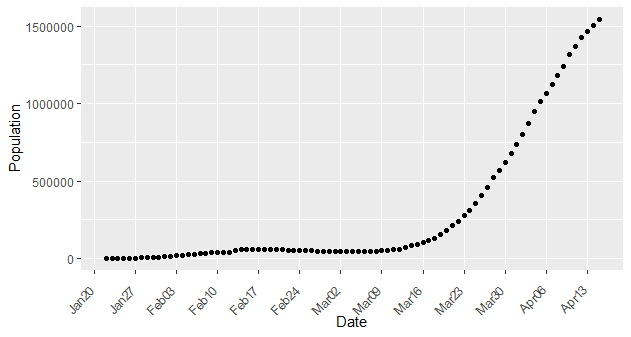
\includegraphics[width=13cm]{P3F1}
	\caption{Number of infections changes over time} \label{P3F1}
\end{figure}\\
4. \textbf{Data integrity analysis: }The completeness of the data is obtained by calculating the proportion of effective values in the data set (Appendix C, lines 87-93). Some results are shown in the Table.\ref{P3T1}(Two ways of merging are given in the code. Scheme one needs to use the primary key generation function written by itself, but the primary key is preprocessed to make the population,latitude and longitude data completeness reach 98.11\% and 98.86\%. The second scheme uses Double key as the primary key, but the completeness of population and latitude and longitude data is 68\%)
% Please add the following required packages to your document preamble:
% \usepackage[table,xcdraw]{xcolor}
% If you use beamer only pass "xcolor=table" option, i.e. \documentclass[xcolor=table]{beamer}
\begin{table}[H]
	\centering
	\caption{Data integrity table} \label{P3T1}              %%%%%%%%%%%%%%%%%%%%%%%%???????????
	\begin{tabular}{lllllllll}
		\hline
		\textbf{Index} & \textbf{Confirmed} & \textbf{Deaths} & \textbf{Recoverd} & \textbf{Date} & \textbf{Country} & \textbf{Increase rate} & \textbf{Population} & \textbf{location} \\ \hline
		Completion         & 99.62\%       & 99.62\%       & 94.69\%       & 100\%         & 100\%         & 99.62\%      & 98.11\%      & 98.86\%      \\ \hline
	\end{tabular}
\end{table}

\noindent \textbf{5. Variable correlation analysis:}For the correlation analysis of variables, generally consider the following methods: 1. Euclidean algorithm 2. Pearson correlation coefficient algorithm 3. Angle cosine formula, where Euclidean algorithm is suitable for data sets with many data attributes, and the cosine formula It is suitable for data with relatively sparse data, and Pearson correlation coefficient algorithm is suitable for data affected by level expansion. Performing a summary operation on the data set can see that Pearson correlation coefficient algorithm is more suitable for correlation analysis of this data set (some variable data There is an order of magnitude difference), the Pearson correlation coefficient is the quotient of the covariance and standard deviation between two variables, and its expression is:correlation coefficient between $P_i$, $P_j$
$$
\begin{aligned}
R_{i,j} & =\frac{P_i-\overline P_i,P_j-\overline P_j}{\|P_i-\overline P_i\|\|P_j-\overline P_j\|}
= \frac{\sum_{m=1}^{n}(P_{im}-\overline P_i)(P_{jm}-\overline P_j)}{\left[ \sum_{m=1}^{n}(P_{im}-\overline P_i)^2 \sum_{m=1}^{n}(P_{jm}-\overline P_j)^2 \right]^{\frac{1}{2}}}\\
& =\frac{E\left[(P_i-\mu P_i)(P_j-\mu P_j)\right]}{\sigma_{P_i}\sigma_{P_j}}
=\frac{cov(P_i,P_j)}{\sigma_{P_i}\sigma_{P_j}}  ,-1\leq R_{i,j}\leq 1
\end{aligned}
$$

\noindent Calculate the Pearson correlation coefficient for some variables (Appendix C, lines 95-107)in Table.\ref{P3T2} and Figure.\ref{P3F2}(Appendix C, lines 109-185):

\begin{table}[H]
	\centering
	\caption{Pearson correlation coefficient} \label{P3T2}
	\begin{tabular}{|l|l|l|l|l|l|}
		\hline
		\textbf{Index}  & \textbf{Date} & \textbf{Confirmed} & \textbf{Recovered} & \textbf{Death} & \textbf{Increase rate} \\ \hline
		\textbf{Date}  & 1           & 0.806501     & 0.840417     & 0.765599     & -0.4506      \\ \hline
		\textbf{Confirmed} & 0.806501    & 1            & 0.806501     & 0.995398     & -0.21135     \\ \hline
		\textbf{Recovered} & 0.840417    & 0.98934      & 1            & 0.988752     & -0.24571     \\ \hline
		\textbf{Death} & 0.765599    & 0.995398     & 0.988752     & 1            & -0.19537     \\ \hline
		\textbf{Increase rate} & -0.4506     & -0.21135     & -0.24571     & -0.19537     & 1            \\ \hline
	\end{tabular}
\end{table}

\begin{figure}[h]
	\small
	\centering
	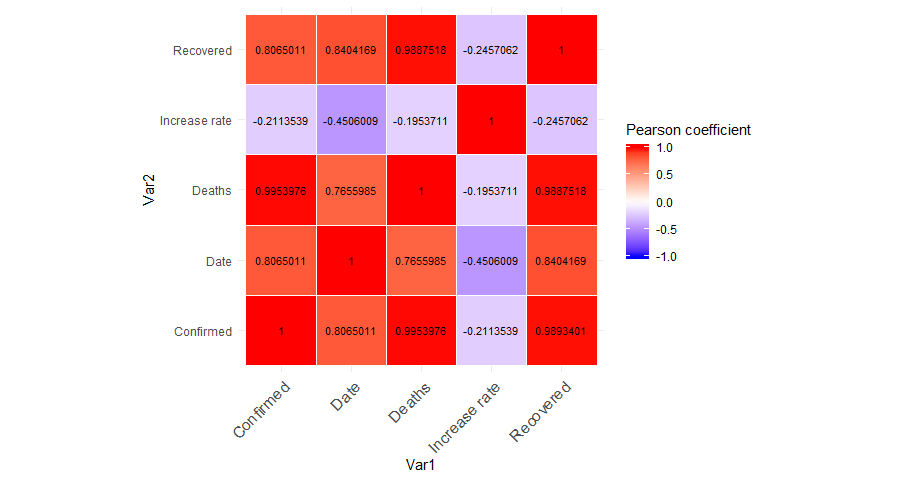
\includegraphics[width=17cm]{P3F2}
	\caption{Correlation coefficient heat map} \label{P3F2}
\end{figure}

\quad According to the obtained correlation coefficient heat map, it can be seen that the greater the number of infected persons, the greater the number of deaths, and the longer the corresponding time; the greater the number of infected persons, the higher the corresponding growth rate, but the growth rate is not related to the remaining variables, only It has a weaker relationship with the duration of the epidemic. These conclusions are basically in line with common sense, and also show that the spread of infectious diseases is related to multiple factors. When analyzing the influencing factors, the influence of multiple factors should be considered\\
6.\textbf{Data normalization: }Because there are different dimensions between the indicators, the data size varies greatly, and the data range is also different, which will increase the difficulty of analysis preprocessing and clustering. Therefore, the index must be normalized and converted into a number between [0,1]. I choose the maximum and minimum method for normalization, and normalize all quantized indexes (Appendix C, lines 187-204),
$$
\begin{aligned}
x_i^{'}=\frac{x_i-x_{min}}{x_{max}-x_{min}}
\end{aligned}
$$

\subsection{Quantitative criteria for analyzing pandemic diseases}
\qquad We need the quantitative conditions that define "epidemic" and "pandemic" diseases through data analysis. Since the current grading of epidemics is still based on qualitative analysis, in order to quantitatively analyze "prevalence" and "pandemic", we need to perform certain mathematical treatments on traditional grading. In epidemiology, the spread of disease can be simply divided into four levels, namely sporadic, outbreak, epidemic and pandemic. "Sporadic" means that there is no temporal or spatial correlation between cases; "outbreak" means that there are many same patients in a collective unit or local area within a short period of time; if the incidence of a disease is significantly higher than usual, It can be considered that the disease is in an "epidemic" state; when the disease spreads rapidly and crosses national boundaries or even continental boundaries in a short time, it can be called a "pandemic." This classification quantifies the epidemic. Based on this category, we can refer to the transmission intensity of major epidemics over the years and start cluster analysis with several evaluation indicators, which are divided into four corresponding categories. Then, based on the classification results, principal component analysis is used to quantitatively distinguish between "popularity" and "pandemic".

\subsubsection{Selection of clustering model}
\qquad Due to the wide variety of evaluation indicators and the complexity of the indicators corresponding to a single infectious disease, I first choose the R-type clustering method to analyze the evaluation indicators, based on the results, and then use the Q-type clustering method to classify the level of infectious diseases and identify their characteristics .

\subsubsection{R-type clustering model establishment}
\qquad R-type clustering is used to reduce dimensionality of indicators. Therefore, we first need to select the indicators that affect the virus's ability to spread. By consulting the literature, I mainly consider 16 well-known infectious diseases, and each infectious disease considers 14 evaluation indicators, namely: comprehensive population of outbreak place, number of infected persons, number of sick and dead, number of cured, duration of epidemic, number of infected countries , The growth rate, the number of basic infections, the mortality rate, the GDP per capita in the outbreak area, the population density in the outbreak area, and the epidemic prevention measures in the outbreak area. The incubation period, the proportion of asymptomatic infections, and the number of basic infections. This cluster introduced a new indicator $R_0$. This indicator indicates the average number of other people infected by a certain infectious disease without the intervention of external forces and the immunity of all people. An important critical point of $R_0$ is $R_0$=1. The larger the number of $R_0$, the harder it is to control the epidemic. For example, when $R_0$ is less than 1, it means that the infectious disease will gradually disappear; when $R_0$ is equal to 1, the infectious disease will become an endemic epidemic; when $R_0$ is greater than 1, the infectious disease will spread exponentially , The data is shown in Appendix A.

\quad The NA means: 1. The data cannot be compared: for example, the GDP of 300 years ago was converted into US dollars and the per capita GDP of a country was converted to US dollars 5 years ago. 2. No data: such as the number of people infected with mumps 3. The data is meaningless: such as the diphtheria virus The carrier will not get sick or be contagious, so the data is meaningless for cluster analysis. 4. The data is not credible: data with large differences found on different websites.

\quad The number of virus infections is once (or the first if data is available for the first time) a pandemic infections. The reason for NA is that the disease is indeed a pandemic, but there are no outbreaks or multiple outbreaks at the same time, or humans have never been eliminated. Such as AIDS

\quad The data is directly removed because it is difficult to quantify the government response. Simultaneous removal the ills always epidemic small-scale outbreaks, such as diphtheria.

\quad Standardize and normalize the data separately (Appendix C, lines 206-242), use the Euclidean distance as the distance when clustering, and use the cluster average clustering method to obtain the Figure.\ref{P3F3} and Figure.\ref{P3F4}(Appendix C, lines 227-242).\\
\begin{figure}[H]
	\small
	\centering
	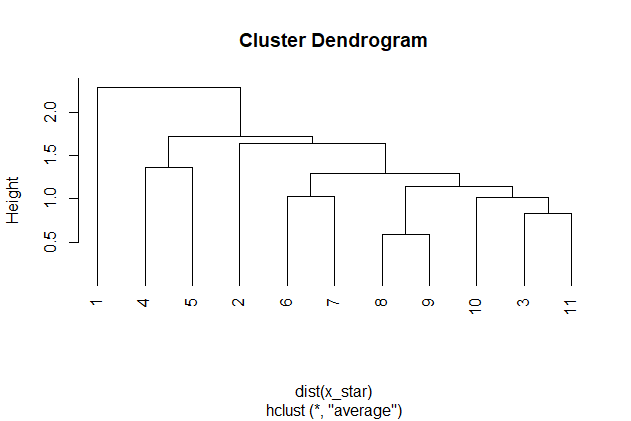
\includegraphics[width=12cm]{P3F4}
	\caption{R-type clustering results after data normalization} \label{P3F3}
\end{figure}
\begin{figure}[h]
	\small
	\centering
	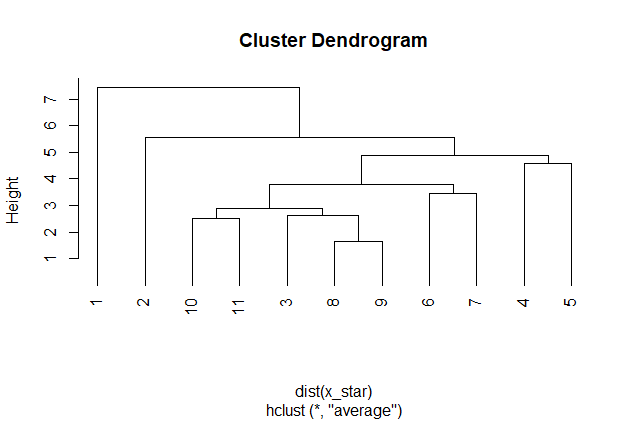
\includegraphics[width=12cm]{P3F3}
	\caption{R-type clustering results after data standardization} \label{P3F4}
\end{figure}
\noindent As can be seen from the Figure.\ref{P3F3} and Figure.\ref{P3F4}, the index 8,9,10,11 have a large correlation and are first brought together. Divide index 18 into 6 categories, each specific indicator and the 6 representative indicators finally determined are shown in Table.\ref{P3T3}
\begin{table}[H]
	\centering
	\caption{Basic information of various categories of indicators} \label{P3T3}
	\begin{tabular}{lll}
		\hline
		\textbf{Serial} & \textbf{Index} & \textbf{Representative index} \\ \hline
		First category      & 1           & Confirmed           \\
		Second category         & 4           & Death rate            \\
		Third category         & 5           & $R_0$             \\
		Fourth category         & 2           & Deaths           \\
		Fifth category         & 6 7         &  Incubation period           \\
		sixth category         & 3 8 9 10 11 &  Explosive place, Number of cured      \\ \hline
	\end{tabular}
\end{table}

\quad From the above results, it can be seen that indicators 1 (number of infected persons), 4 (case fatality rate), 5 ($R_0$), and 2 (number of deaths) are different from other types of diseases, each of which is a separate category; the sixth category contains There are many indicators 3 (cure rate), 8 (proportion of asymptomatic infections), 9 (duration), 11 (outbreak information), indicating that these types of indicators have certain internal links. In general, the number of basic infections and the case fatality rate directly affect the harmfulness of infectious diseases. The epidemic prevention measures at the outbreak site are related to the duration of infectious diseases. These understandings are reflected in the classification results, which also shows that the results have better adaptability to the problem. related. These understandings are reflected in the classification results, which also shows that the results have better adaptability to the problem.\\

\subsubsection{Q-type clustering model establishment}
\qquad Based on the conclusions drawn above, Q-type cluster analysis was used to classify 15 classic infectious diseases.\\
1. \textbf{Sample similarity index}

\quad To classify things in a quantitative way, we must describe the degree of similarity between things in a quantitative way. The sample points to be classified need to be described with $p$ variables, so each sample point can be regarded as a point in the $R_p$ space. Therefore, it is natural to think that distance can be used to measure the similarity between sample points. Here I use the Min distance to calculate and solve. The Min distance is calculated as follows:
$$
\begin{aligned}
\centering
d_{ij}(q)=\left( \sum_{k=1}^p \left|X_{ik}-x_{jk}\right|^q \right)^{\frac{1}{q}}
\end{aligned}
$$
Here we use q=2, which is the Euclidean distance\\
2.\textbf{Similarity measure between classes}

\quad I use the inter-class average connection method for system clustering. The inter-class average connection method defines the square of the distance between the classes as the average of the distance squared between the elements in the two classes. For any class, the similarity between $G_k$ and $G_r$ is :

$$
\begin{aligned}
\centering
D_{kr}^2=\frac{n_p}{n_r}D_{kp}^2+\frac{n_q}{n_r}D_{kq}^2
\end{aligned}
$$

\quad Similar to the R-type clustering code(Appendix C, lines 224-250), result is Figure\ref{sp1}:
\begin{figure}[h]
	\small
	\centering
	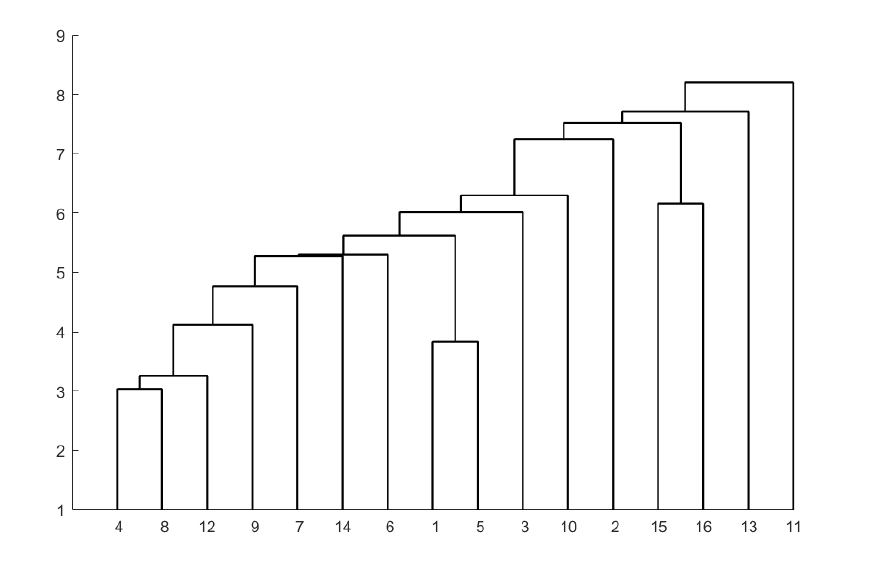
\includegraphics[width=11cm]{sp1}
	\caption{Q-type clustering results after data normalization} \label{sp1}
\end{figure}
\begin{table}[H]
	\centering
	\caption{Basic information on various types of illness} \label{P3T4}
	\begin{tabular}{llll}
		\hline
		\textbf{Serial} & \textbf{Infectious Disease Code}          & \textbf{Representative value} & \textbf{level} \\ \hline
		First category         & 11                      & Pertussis          & Sporadic          \\
		Second category         & 13                      & Mumps          & outbreak        \\
		Third category         & 4,8,12,9,7,6,1,5,3,10,2 & Measles           & Epidemic          \\
		Fourth category         & 15,16                   & COVID-19     & Pandemic         \\ \hline
	\end{tabular}
\end{table}
\quad It can be seen from the Figure.\ref{sp1}, Table.\ref{P3T4} that the infectious diseases 11 (pertussis) and 13 (mumps) are divided into one category, and the transmission levels are "sporadic" and "outbreak", respectively. Disease 15 (type A H1N1), 16 (COVID-19) are divided into one category, the transmission level is "pandemic", the fourth category covers most infectious diseases (>50\%), and the transmission level is "epidemic" . By referring to relevant information, pertussis is an acute respiratory infectious disease, but it can rarely be transmitted through external conditions, so it is classified as a category; and influenza can cause a large spread, but the transmission route is easy to block , Wearing a mask), and the case fatality rate is low, the degree of harm is small, and it is classified as a class; A H1N1 and COVID-19 have a strong spreading ability, a high mortality rate, a large number of transmission routes, and a large degree of influence. As a category, the classification results are consistent with the conclusions given by the World Health Organization (WHO). This is consistent with our understanding, and also shows that this model has a higher accuracy.

\subsubsection{Establishment of comprehensive evaluation model}
\qquad Through clustering analysis, 16 types of infectious diseases were included into 4 types, and 6 types of indicators affecting interaction were selected from 14 types of indicators. According to different categories, we use a comprehensive evaluation model to score different categories of infectious diseases to achieve a quantitative division of categories. Subdivided by quantitative indicators and data decomposition, we replace the principal component analysis model as an infectious disease classification evaluation model. Evaluation indicators are: number of infections, mortality rate, $R_0$, number of deaths, incubation period, outbreak site, number of cured

\quad The standard method using principal component analysis: 1. Data standardization 2. Calculate the correlation coefficient matrix R 3. Find the eigenvalues and eigenvectors 4. Calculate the contribution rate of the eigenvalues 5. Sort the different infectious diseases to get the epidemiological judgment Mathematical boundary.(Appendix C lines 252-293) The cumulative contribution value of the principal component is finally obtained, the table\ref{P3T5} and the Figure\ref{P3F5}

\begin{table}[H]
	\centering
	\caption{Contribution rate and cumulative contribution rate results} \label{P3T5}
	\begin{tabular}{llll}
		\hline
		\textbf{Index} & \textbf{Eigenvalues} & \textbf{Contribution rate} & \textbf{Cumulative contribution rate} \\ \hline
		1           & 44.1742      & 0.4417       & 0.4417         \\
		2           & 23.8824      & 0.2388       & 0.6806         \\
		3           & 16.3155      & 0.1632       & 0.8437         \\
		4           & 9.1831       & 0.0918       & 0.9356         \\
		5           & 4.7594       & 0.0486       & 0.9842         \\
		6           & 1.6052       & 0.0158       & 1              \\ \hline
	\end{tabular}
\end{table}

\begin{figure}[h]
	\small
	\centering
	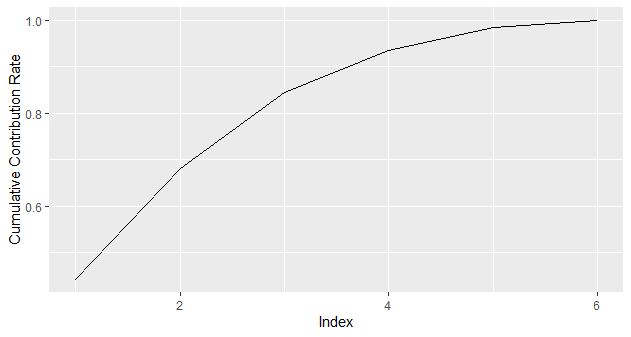
\includegraphics[width=12cm]{P3F5}
	\caption{Principal component cumulative contribution rate distribution} \label{P3F5}
\end{figure}
\begin{table}[]
	\centering
	\begin{tabular}{lll}
		\hline
		\textbf{Serial} & \textbf{Index} & \textbf{Representative value} \\ \hline
         first category        & 1           & Confirmed           \\
         second category        & 4           & Death Rate            \\
         third category        & 5           & $R_0$             \\
         fourth category       & 2           & Deaths           \\ \hline
	\end{tabular}
\end{table}

\quad As shown in Table.\ref{P3T5}, figure\ref{P3F5}, it can be seen that the cumulative contribution rate has exceeded 90\% when $4\leq p$, so the first four sets of indicator variables are used instead of 6 indicators for analysis. The main component comprehensive evaluation model is :
$$
Z=0.4417y_1+0.2388y_2+0.1632y_3+0.0918y_4
$$

\quad According to the normalization of the scoring results, four types of comprehensive scores are obtained, and the score distribution chart is drawn as shown in Figure\ref{P3F6}:
\begin{figure}[H]
	\small
	\centering
	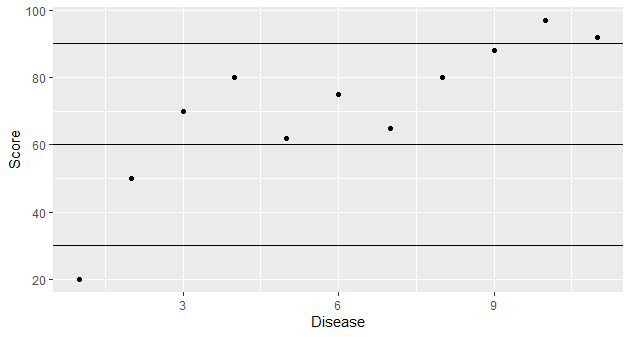
\includegraphics[width=12cm]{P3F6}
	\caption{Distribution of comprehensive scores of various infectious diseases} \label{P3F6}
\end{figure}

\quad We can see that when the normalized score is in the interval [0,30], the corresponding propagation type is "dissemination", and when the normalized score is in the interval (30,60], the corresponding propagation type is "outbreak", and the normalized score In the interval (60, 90), the corresponding type of transmission is "epidemic", and the normalized score is in the interval (90, 100), the corresponding type of transmission is "pandemic." The infectious diseases mentioned in question 1 are all spread more widely Diseases, of which H1N1 and COVID-19 have the greatest impact on human economic production, so they are classified as "pandemic" transmission levels. The results of this classification are in line with our understanding and are reasonable.

\subsection{Using the improved SEIR model to predict the number of asymptomatic infections}
\qquad Virus propagation dynamics models generally include S-DI-A model of multi-group propagation, SIS epidemic model with impulse, SIQS with ordinary differential equations, SEIR model, and SIRS model with time delay. I chose the more general SEIR model\\
1.\textbf{SI model}
\begin{figure}[H]
	\small
	\centering
	
\includegraphics[width=8.5cm]{E1}
	\caption{SI model} \label{C1}
\end{figure}
\quad The SI model divides the population into two types, one is a susceptible person, and the susceptible person is a healthy population, using $S$ to represent the number of people, and the other is an infected person, that is, the patient, the number is represented by $I$. Let's assume that the total number of people in an area is $N$ and then $N=S+I$. If $I$ infected people are not effectively quarantined, each person encounters r people every day, and there is a probability of $\beta$ infection. The proportion of healthy people is $\frac {S}{N}$, and the above variables are multiplied to be the number of new cases per day. The differential equation is as follows
$$
\begin{aligned}
\frac{dI}{dt}&=\frac{r\beta IS}{N}    \\
\frac{dS}{dt}&=-\frac{r\beta IS}{N}
\end{aligned}
$$
Can use R language to easily calculate the predicted value
$$
\begin{aligned}
I_n&=I_{n-1}+\frac{r\beta {I_n}-1S{n-1}}{N}    \\
S_n&=S_{n-1}-\frac{r\beta {	I_n}-1S{n-1}}{N}
\end{aligned}
$$\\
2.\textbf{SIS model}
\begin{figure}[H]
	\small
	\centering
	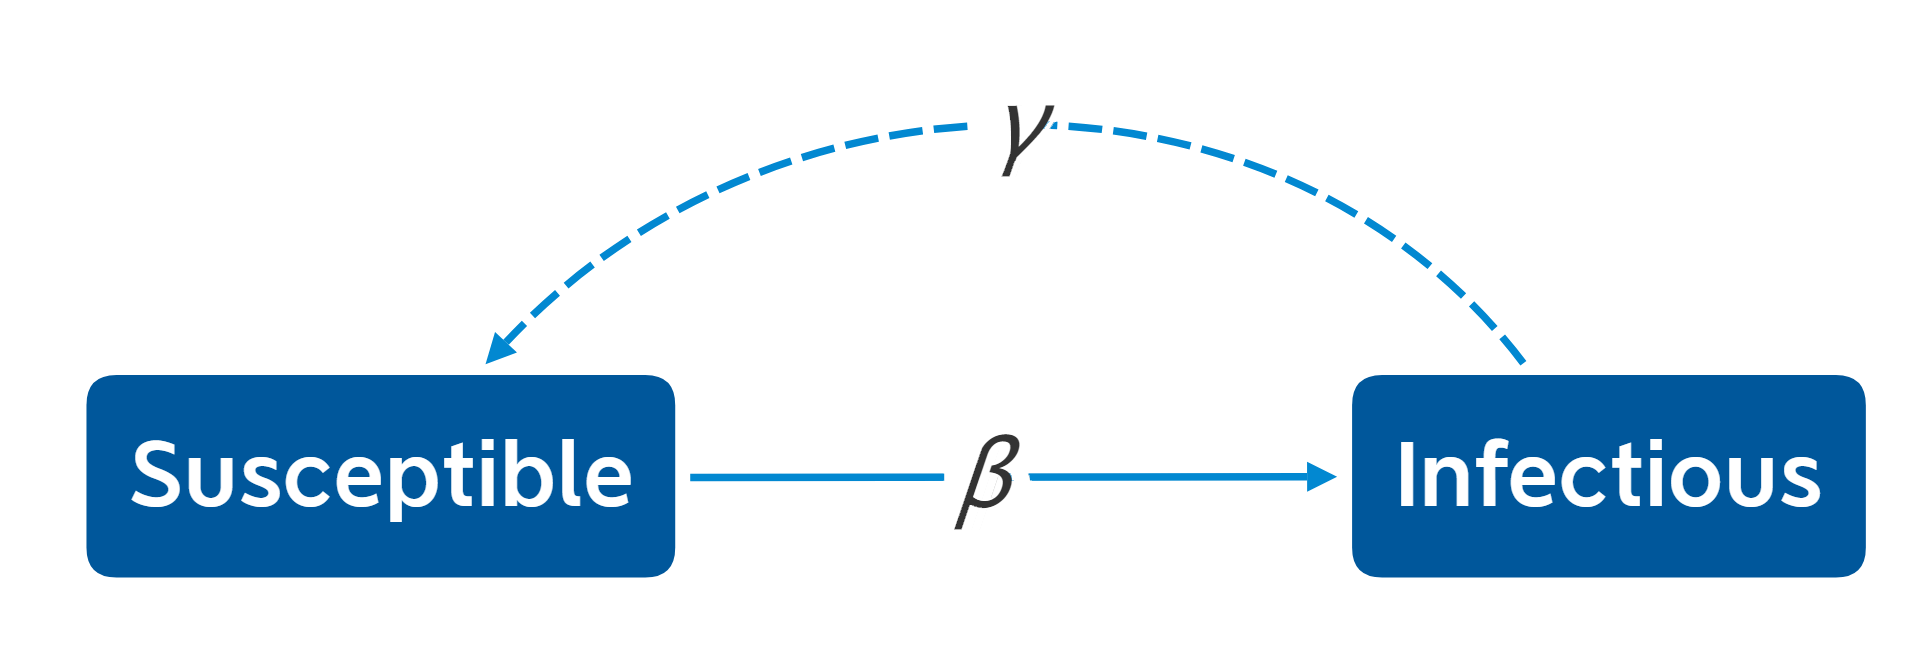
\includegraphics[width=8.5cm]{E2}
	\caption{SIS model} \label{C2}
\end{figure}
\noindent Improve the SI model, think that some people are cured but will still be infected repeatedly, similar to the spread of influenza.\\
Such a model is the SIS model. The SIS model has an additional probability of the infected person $I$ recovering health $\gamma$ than the SI model. Add to the differential equation again:
$$
\begin{aligned}
\frac{dI}{dt}&=\frac{r\beta IS}{N}-\gamma I\\
\frac{dS}{dt}&=-\frac{r\beta IS}{N}+\gamma I\\
\end{aligned}
$$
The iterative equation is modified to

$$
\begin{aligned}
I_n&=I_{n-1}+\frac{r\beta I_{n-1}S_{n-1}}{n}-\gamma I  \\
S_n&=S_{n-1}-\frac{r\beta I_{n-1}S_{n-1}}{n}+\gamma I
\end{aligned}
$$\\
3.\textbf{SIR model}
\begin{figure}[H]
	\small
	\centering
	
\includegraphics[width=11cm]{E3}
	\caption{SIR model} \label{C3}
\end{figure}
\quad Improve the SI model and consider that people who develop antibodies after recovery will not get sick again. Unlike the SIS model, we introduce the rehabilitation person in the model, denoted by R, and satisfy the total number N=S+I+R. This time is the SIR model. Once it becomes a recovered person, there will be no further infection, that is, in the process of probability transmission, once it becomes a recovered person, there is no probability to transfer to an infected or susceptible person again. We assume that the probability of an infected person becoming a recovered person is $\gamma $, and the differential equations listed:
$$
\begin{aligned}
\frac{dS}{dt}&=\frac{-r\beta IS}{N}  \\
\frac{dI}{dt}&=\frac{r\beta IS}{N}-\gamma I \\
\frac{dR}{dt}&=\gamma I
\end{aligned}
$$
\noindent The iterative equation is modified to
$$
\begin{aligned}
S_n&=S_{n-1}-\frac{r\beta I_{n-1}S_{n-1}}{N}  \\
I_n&=I_{n-1}+\frac{r\beta I_{n-1}S_{n-1}}{N}-\gamma I_{n-1}  \\
R_n&=R_{n-1}+\gamma I_{n-1}
\end{aligned}
$$\\
4.\textbf{SEIR model}
\begin{figure}[H]
	\small
	\centering
	
\includegraphics[width=13cm]{E4}
	\caption{SEIR model} \label{C4}
\end{figure}
\quad The actual situation is more complicated. The susceptible people will experience the incubation period (asymptomatic infection period) at the beginning, and the symptoms will appear after a period of time. Therefore, we introduced the latent person (asymptomatic infected person) based on the SIR model. The probability $\alpha$ is transformed into an infected person, and the differential equation is modified on the basis of SIR:
$$
\begin{aligned}
\frac{dS}{dt}&=-\frac{r\beta IS}{N}\\ 
\frac{dE}{dt}&=\frac{r\beta IS}{N}-\alpha E\\ 
\frac{dI}{dt}&=\alpha E-\gamma I\\ 
\frac{dR}{dt}&=\gamma I
\end{aligned}
$$
\noindent The iterative equation is modified to:
$$
\begin{aligned}
S_n&=S_{n-1}-\frac{r\beta I_{n-1}S_{n-1}}{N}\\ 
E_n&=E_{n-1}+\frac{r\beta I_{n-1}S_{n-1}}{N}-\alpha E_{n-1}\\ 
I_n&=I_{n-1} +\alpha E_{n-1}-\gamma I_{n-1}\\ 
R_n&=R_{n-1}+\gamma I_{n-1}
\end{aligned}
$$

\subsubsection{Improvement of SEIR model in COVID-19 (Chongqing as an example)}
\qquad We found that in the COVID-19 epidemic, asymptomatic infected persons (latent persons) are infectious during the incubation period of the virus, so we have to introduce the infection probability of latent persons $\beta_2$ can transform healthy people into asymptomatic infected persons (latent By). The number of healthy susceptible people who are exposed to asymptomatic infections every day is $r_2$. The differential equation obtained is:

$$
\begin{aligned}
\frac{dS}{dt}&=-\frac{r\beta IS}{N}-\frac{r_2 \beta_2ES}{N} \\
\frac{dE}{dt}&=\frac{r\beta IS}{N}-\alpha E+\frac{r_2 \beta_2ES}{N}  \\ 
\frac{dI}{dt}&=\alpha E-\gamma I  \\ 
\frac{dR}{dt}&=\gamma I
\end{aligned}
$$
\noindent The iterative equation is modified to:
$$
\begin{aligned}
S_n&=S_{n-1}-\frac{r\beta I_{n-1}S_{n-1}}{N}-\frac{r_2\beta_2 E_{n-1}S_{n-1}}{N}  \\
E_n&=E_{n-1}+\frac{r\beta I_{n-1}S_{n-1}}{N}-\alpha E_{n-1}+\frac{r_2\beta_2 E_{n-1}S_{n-1}}{N}  \\ 
I_n&=I_{n-1} +\alpha E_{n-1}-\gamma I_{n-1}  \\ 
R_n&=R_{n-1}+\gamma I_{n-1}
\end{aligned}
$$

\quad We substituted the number of infected people in Chongqing into the model and found that no matter how the parameters were modified, the difference between the predicted value and the actual value in the first few days was small, but the gap became larger with time. I think it is because: 1. The $S$  in model is susceptible, not all populations. 2. When the virus outbreaks in a certain city, the city will take anti-epidemic measures, and the value of $r$ and $r_2$ will drop instantly. 3. Rehabilitation rate increases with time (if we learn from the experience of other cities, it will increase instantly). So add two conditions to predict again (Appendix C, lines 296-343) result shown in Figure.\ref{P3F7})\\
\vspace{-0.5cm}
\begin{figure}[H]
	\small
	\centering
	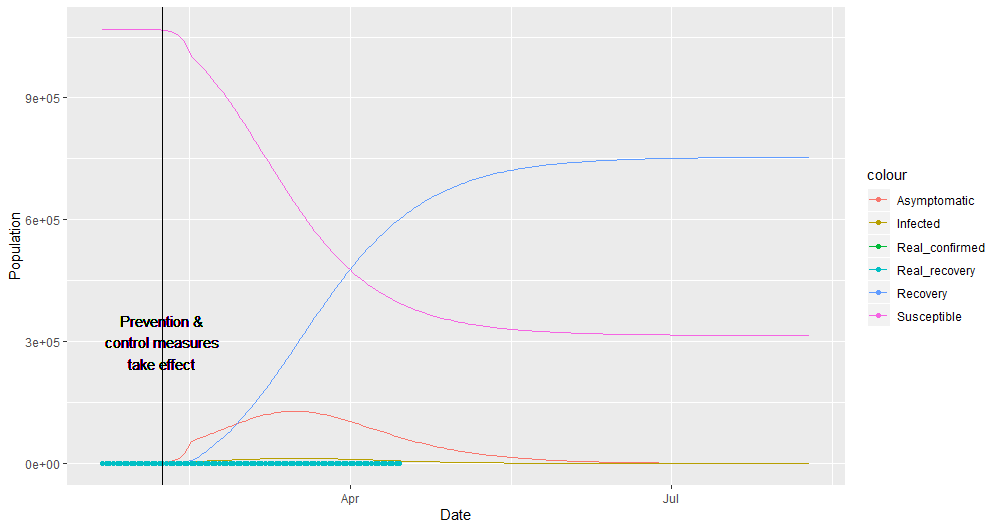
\includegraphics[width=12cm]{P3F7}
	\caption{The prediction result of the first improvement of the SEIR model} \label{P3F7}
\end{figure}

\begin{figure}[H]
	\small
	\centering
	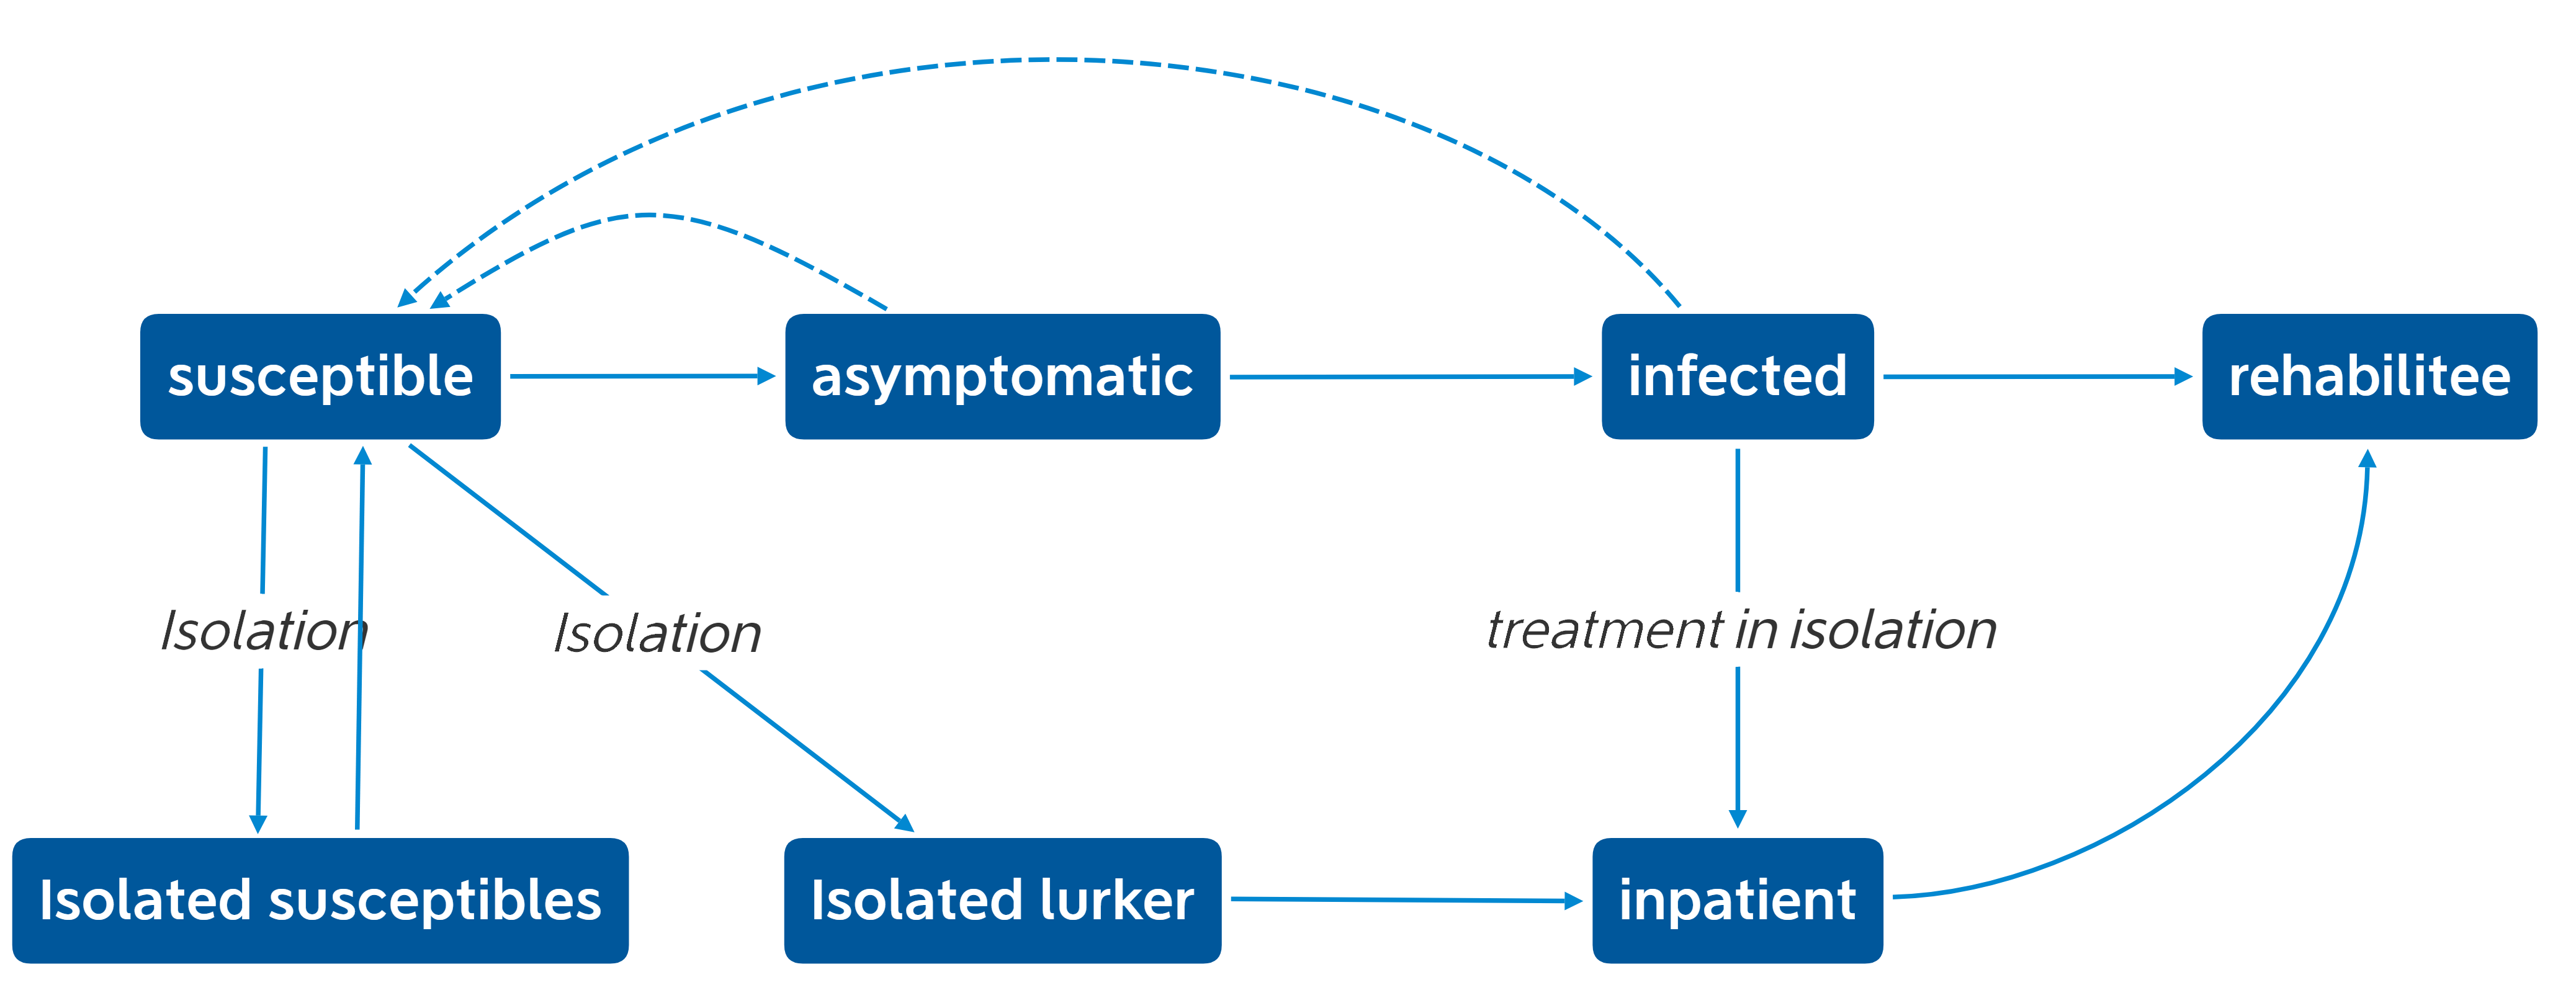
\includegraphics[width=14cm]{E5}
	\caption{SEIR model second improvement} \label{C5}
\end{figure}

\quad Support: The isolation ratio is $ q $, the infection probability is $ \ beta $, the contact cures $ c $, and $ \ rho $ is the effective contact coefficient. The reference value of the effective contact coefficient is 1, and $ \ rho c $ is the effective contact rate. The susceptible $ S $ to isolate the susceptible $ S_q $, the isolation lurking $ E_q $, the lurking $ E $ conversion rate is $ \ rho cq (1- \ beta) $, $ \ rho cq \ beta $ And  $ rho c \ beta(1-q)$. At the same time, considering the impact of non-isolated infected persons $I$ and latent persons $E$ on susceptible people, and quarantined susceptible persons who have been released from isolation $S_q$ is converted back to $S$, so the control equation for the number of susceptible persons is
$$
\frac{dS}{st}=S(1+\theta E)\left[ \rho c \beta + \rho cq(1-\beta) \right]+\lambda S_q
$$

\quad Among them, $\theta$ is the ratio of asymptomatic infected persons to the spreading ability of general infected persons. We assume that the spreading ability is the same at the beginning of virus transmission, that is, $\theta =1$. $\lambda$ is the isolation release rate. Take $\lambda=\frac{1}{14}$ (isolation time is 14 days). So the differential equation of the new SEIR model is constructed:

$$
\begin{aligned}
\frac{dS}{st}&=S(1+\theta E)\left[ \rho c \beta + \rho cq(1-\beta) \right]+\lambda S_q \\
\frac{dE}{dt}&=\rho c \beta (1-q)S(I+\theta E)-\sigma E \\
\frac{dI}{dt}&=\sigma E-\left( \delta_I +\alpha +\gamma_I \right)I \\
\frac{dS_q}{dt}&=\rho c q(1-\beta)S(I+\theta E)-\lambda S_q \\
\frac{dE_q}{dt}&=\rho c \beta q S(I+\theta E)-\delta_qE_q \\
\end{aligned}
$$
$$
\begin{aligned}
\frac{dH}{dt}&=\delta_II+\delta_qE_q-\left( \alpha + \gamma_H \right)H \\
\frac{dR}{dt}&=\gamma_II+\gamma_HH
\end{aligned}
$$

\quad I used the data from Chongqing as a query set to understand the different parameters and analyze the changes in the resulting image to get the specific values of the parameters (Appendix C, lines 364-376). The data of the number of infected people in Hubei Province was tested as a test set (Appendix C, lines 347-425) to obtain the Figure.\ref{P3F8}, Figure.\ref{P3F9}

\begin{figure}[H]
	\small
	\centering
	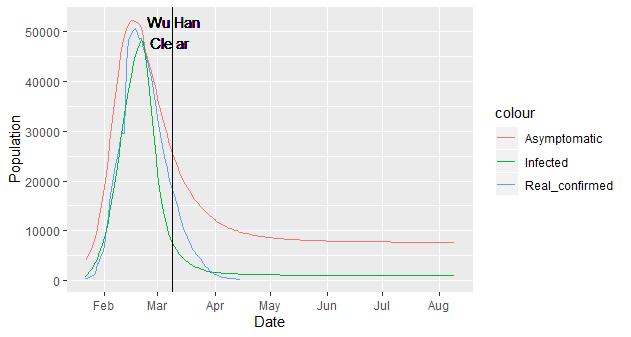
\includegraphics[width=16.5cm]{P3F8}
	\caption{Compare the number of infected people with the actual number of people after the second improvement of the SEIR model and predict the number of asymptomatic infected people} \label{P3F8}
\end{figure}

\begin{figure}[H]
	\small
	\centering
	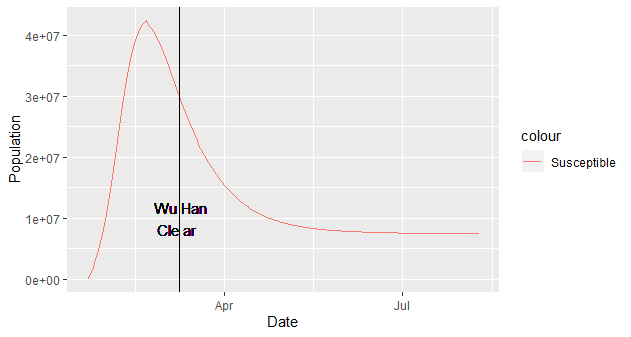
\includegraphics[width=13cm]{P3F9}
	\caption{Changes in the number of susceptible people after the second improvement of the SEIR model} \label{P3F9}%%%%%%%%%%??????????????????????????
\end{figure}

\subsubsection{Result analysis}
\qquad It can be seen that the curve is divided into three stages. The first stage is the early rising stage: it belongs to the early stage of the virus outbreak, the number of latent people (asymptomatic infections) has risen rapidly, and the number of asymptomatic infections has also continued to rise; the second stage is the mid-term regulation stage, which was implemented at the beginning of this stage. Although the number of asymptomatic people has increased in urban isolation, mask wearing, treatment and other measures, the late stage has been controlled and reached a peak after about 22 days; the third stage is the late stage of decline. This stage is due to the continuous implementation of the previous measures, asymptomatic infection The downward trend of the number is obvious. Within 140 days after the beginning of the epidemic, the number of newly-increased asymptomatic infections per day will drop to zero, that is to say, by mid-May, the number of newly-increased asymptomatic infections in Hubei will approach zero.

\quad The number of asymptomatic infections is between 4.15 and 8.9. The number of asymptomatic infections is predicted as Appendix B.

\subsection{Verification of SEIR model using response surface prediction model}
\qquad When the number of asymptomatic infections changes, the SEIR model we use belongs to the virus transmission dynamics model. We can also predict the number of asymptomatic infections through statistical models, so I use the response surface prediction model to predict the number of asymptomatic infections to verify the correctness of the improved SEIR model

\quad I used the number Y of asymptomatic infections as the dependent variable, and selected 4 typical indicators based on the R-type clustering results: the number of patients P, the number of basic infections $R_0$, the incubation period T, and the cure rate $R_c$ four indicators. To predict the development trend of the number of asymptomatic infections, we plan to use a response surface prediction model to establish the relationship between Y and the four indicators.

\quad Response surface design method, through designing reasonable test method and obtaining test result data through reasonable operation, using multiple quadratic linear regression method to establish the functional relationship between independent variable and response value, and analyzing the change trend of response value through regression equation , This method is more common in solving multivariate problems.

\quad Due to the complexity of response surface prediction in R language, I used the experimental design software Design-Expert and chose the BBD experimental design method. Response surface refers to the functional relationship between response variable (dependent variable) Y and a set of input variables $x_i$.

\quad In the experiment, the response variable was the number of asymptomatic infections Y, and the independent variable considered four factors: P, $R_0$, T, and $R_c$. Design-Expert conducted a total of 29 sets of experiments and obtained the Table\ref{P3T8}

\begin{table}[H]
	\centering
	\caption{The five best experiments} \label{P3T8}
	\begin{tabular}{llllll}
		\hline
		\textbf{experiment} & \textbf{P} & \textbf{$R_0$} & \textbf{T} & \textbf{$R_c$} & \textbf{Y} \\ \hline
		experiment1         & 2.75       & 5              & 12.5       & 0.2            & 2202       \\
		experiment2         & 5          & 3              & 12.5       & 1              & 1971       \\
		experiment3         & 0.5        & 3              & 20         & 0.6            & 1325       \\
		experiment4         & 0.5        & 3              & 5          & 0.6            & 883        \\
		experiment5         & 2.75       & 3              & 12.5       & 0.6            & 1243       \\ \hline
	\end{tabular}
\end{table}

\noindent So we build a quadratic polynomial model of the response surface

$$
\begin{aligned}
y=1.65+0.35P+0.57R_0+0.1T-0.55R_c+0.16PR_0-0.11PT+0.15PR_c \\
-0.04R_0T+0.14R_0R_c+0.02P^2+0.09R_0^2-0.18T^2-0.05R_c^2
\end{aligned}
$$

\noindent Draw an image of the number of asymptomatic infections over time:Figure.\ref{res}

\begin{figure}[]
	\small
	\centering
	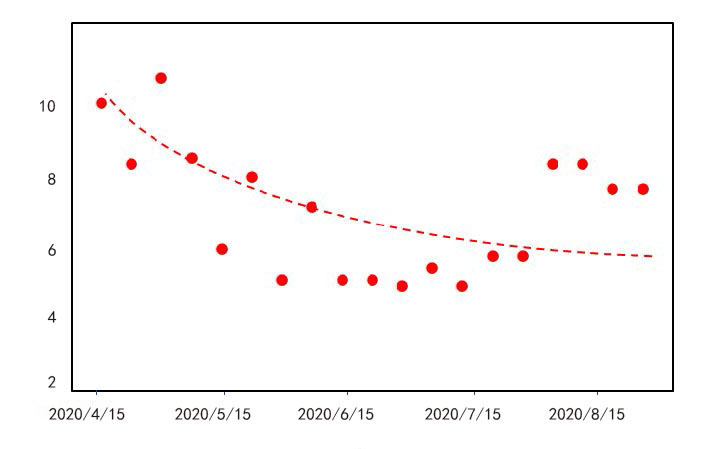
\includegraphics[width=11cm]{res}
	\caption{Predicting the number of asymptomatic infections} \label{res}
\end{figure}

\quad In the process of response surface analysis, the F value is used to detect the significance of statistical results, and the p value is used to detect the significance of the regression coefficient. The smaller the p value, the more significant the result. The results are shown in the table. From the Table.\ref{P3T9}, the model F value is 5.37, p<0.05, indicating that the model has significant adaptability, and the relationship between each factor and the response value in the regression equation is significant.

\begin{table}[]
	\centering
	\caption{Response surface analysis table} \label{P3T9}
	\begin{tabular}{llllll}
		\hline
		\textbf{parameter}  & \textbf{sum of square} & \textbf{Degrees of freedom} & \textbf{Mean square} & \textbf{F} & \textbf{p}     \\ \hline
		\textbf{model}  & 9.84         & 14           & 0.70        & 5.37         & 0.0017(*)       \\
		\textbf{A}   & 1.48         & 1            & 1.48        & 11.29        & 0.0047           \\
		\textbf{B}   & 3.91         & 1            & 3.91        & 29.93        & \textless 0.0001 \\
		\textbf{C}   & 0.13         & 1            & 0.13        & 0.98         & 0.3387           \\
		\textbf{D}   & 3.68         & 1            & 3.68        & 28.10        & 0.0001           \\
		\textbf{Residual}  & 1.83         & 14           & 0.13        &              &                  \\
		\textbf{Net error} & 0.23         & 4            & 0.059       &              &                  \\
		\textbf{Net error} & 11.67        & 28           &             &              &                  \\ \hline
	\end{tabular}
\end{table}

\noindent So far we have verified the correctness of the improved SEIR model.

\quad This disaster that has swept the world has made us re-recognize our self-confidence, perseverance, will, and mutual help... Data scientists used various models to predict the development trend of the virus in the first time, and played an important role in the prevention and control of the epidemic. But the most important thing is that \textbf{we firmly believe that there will be no difficulties that can defeat us. We firmly believe that ice and snow will eventually melt, and spring will come as scheduled. Our country is blooming in spring.}

\newpage
\begin{thebibliography}{99}
	\addcontentsline{toc}{subsection}{Reference}
	\bibitem{1}Weiss, R. A., \& McMichael, A. J. (2004). Social and environmental risk factors in the emergence of infectious diseases. Nature medicine, 10(12 Suppl), S70–S76. https://doi.org/10.1038/nm1150
	\bibitem{2}Tang, B., Wang, X., Li, Q., Bragazzi, N. L., Tang, S., Xiao, Y., \& Wu, J. (2020). Estimation of the Transmission Risk of the 2019-nCoV and Its Implication for Public Health Interventions. Journal of clinical medicine, 9(2), 462. https://doi.org/10.3390/jcm9020462
	\bibitem{3}Wu, J. T., Leung, K., \& Leung, G. M. (2020). Nowcasting and forecasting the potential domestic and international spread of the 2019-nCoV outbreak originating in Wuhan, China: a modelling study. The Lancet, 395(10225), 689-697.
	\bibitem{4}Weiss RA, McMichael AJ. Social and environmental risk factors in the emergence of infectious diseases. Nature Medicine. 2004 Dec;10(12 Suppl):S70-6. DOI: 10.1038/nm1150.
	\bibitem{5}Mutreja, A., Kim, D. W., Thomson, N. R., Connor, T. R., Lee, J. H., Kariuki, S., ... \& Niyogi, S. K. (2011). Evidence for several waves of global transmission in the seventh cholera pandemic. Nature, 477(7365), 462-465.
	\bibitem{6}Murray, C. J., Lopez, A. D., Chin, B., Feehan, D., \& Hill, K. H. (2006). Estimation of potential global pandemic influenza mortality on the basis of vital registry data from the 1918–20 pandemic: a quantitative analysis. The Lancet, 368(9554), 2211-2218.
	\bibitem{7}World Health Organization. 2018. Pandemic Preparedness. [online] Available at: <https://www.who.int/influenza/preparedness/pandemic/en/> [Accessed 13 June 2020].
	\bibitem{8}Hou, C., Chen, J., Zhou, Y., Hua, L., Yuan, J., He, S., ... \& Zhang, J. (2020). The effectiveness of quarantine of Wuhan city against the Corona Virus Disease 2019 (COVID‐19): A well‐mixed SEIR model analysis. Journal of medical virology.
	\bibitem{9}Zou, Y., Pan, S., Zhao, P., Han, L., Wang, X., Hemerik, L., ... \& van der Werf, W. (2020). Outbreak analysis with a logistic growth model shows COVID-19 suppression dynamics in China. medRxiv
\end{thebibliography}

\newpage
\subsection*{Appendix}
\addcontentsline{toc}{subsection}{Appendix}
\subsubsection*{Appendix A: Summary of outbreaks of 15 common infectious diseases}
\begin{table}[H]
	\begin{tabular}{lllllll}
		\hline
		\textbf{Disease\_Name} & \textbf{Confirmed} & \textbf{Deaths} & \textbf{Recovered} & \textbf{Death\_Rate} & \textbf{R0\_min} & \textbf{R0\_max} \\ \hline
		Hepatitis B            & 300000000          & 17000           & 2999998300         & 0.000005             & 1                & 2                \\
		Black Death            & 85000000           & 78700000        & 6300000            & 0.9258               & 1                & 3                \\
		cholera                & 461783             & 8072            & 453711             & 0.0068               & 1                & 2                \\
		measles                & 250270             & 5110            & 245160             & 0.0020               & 12               & 18               \\
		diphtheria             & 2839               & 67              & 2772               & 0.0235               & 6                & 7                \\
		smallpox               & 6000               & 850             & 5150               & 0.3                  & 5                & 7                \\
		polio                  & NA                 & NA              & NA                 & NA                   & 5                & 7                \\
		rubella                & NA                 & NA              & NA                 & 0.0013               & 5                & 7                \\
		Mumps                  & NA                 & NA              & NA                 & 0.0002               & 5                & 7                \\
		HIV/AIDS               & NA                 & NA              & NA                 & NA                   & 2                & 5                \\
		pertussis              & 75598200           & 5292            & 75592908           & 0.00007              & 4                & 7                \\
		SARS                   & 8422               & 919             & 7503               & 0.17                 & 0.85             & 3                \\
		MERS                   & 1139               & 431             & 708                & 0.37                 & 1                & 2                \\
		HIN1                   & 25449514           & 19449           & 25430065           & 0.012                & 1.75             & 1.75             \\
		COVID-19               & 7221717            & 411818          & 6809899            & 0.05                 & 3.77             & 3.77             \\ \hline
	\end{tabular}
\end{table}

\begin{table}[H]
	\begin{tabular}{lllll}
		\hline
		\textbf{Disease\_Name} & \textbf{incubation} & \textbf{Rate\_asymptomatic} & \textbf{Date} & \textbf{Country\_Rate} \\ \hline
		Hepatitis B            & 70                  & 0                           & 8030          & 1                      \\
		Black Death            & 3                   & 0.12                        & 2555          & 1                      \\
		cholera                & 2                   & 0.07                        & 1277          & 1                      \\
		measles                & 10                  & 0.08                        & 317           & 0.025                  \\
		diphtheria             & 3                   & 0.11                        & 115           & 0.01                   \\
		smallpox               & 14                  & 0                           & 730           & 1                      \\
		polio                  & 11                  & 0                           & NA            & 1                      \\
		rubella                & 11                  & 0.01                        & NA            & NA                     \\
		Mumps                  & 19                  & 0.06                        & NA            & NA                     \\
		HIV/AIDS               & 11                  & 0.04                        & NA            & 1                      \\
		pertussis              & 13                  & 0.09                        & 183           & 1                      \\
		SARS                   & 7                   & 0.11                        & 270           & 0.162                  \\
		MERS                   & 5.2                 & 0.18                        & 218           & 0.061                  \\
		HIN1                   & 4                   & 0.19                        & 485           & 1                      \\
		COVID-19               & 14                  & 0.17                        & 190           & 1                      \\ \hline
	\end{tabular}
\end{table}
\begin{table}[H]
	\begin{tabular}{lllll}
		\hline
		Disease\_Name & Origin\_City\_Population & GDP   & Density\_People & Act\_Gov \\ \hline
		Hepatitis B   & 15305900                 & 21874 & 2059            & NA       \\
		Black Death   & 70000000                 & 31058 & 16              & 0        \\
		cholera       & 7510100                  & 3894  & 554             & NA       \\
		measles       & 1800000                  & 3198  & 1772            & NA       \\
		diphtheria    & 257740000                & 3894  & 554             & NA       \\
		smallpox      & 11000                    & 46170 & 963             & NA       \\
		polio         & NA                       & NA    & NA              & NA       \\
		rubella       & NA                       & NA    & NA              & NA       \\
		Mumps         & NA                       & NA    & NA              & NA       \\
		HIV/AIDS      & NA                       & NA    & NA              & NA       \\
		pertussis     & 8900000                  & 46500 & 4761            & NA       \\
		SARS          & 7251900                  & 7404  & 975             & NA       \\
		MERS          & 436000                   & 25059 & 965             & NA       \\
		HIN1          & 38310000                 & 49911 & 90              & NA       \\
		COVID-19      & 12212000                 & 21098 & 2334            & 1        \\ \hline
	\end{tabular}
\end{table}


\newpage
\subsubsection*{Appendix B: Improved SEIR model to predict the number of asymptomatic infected persons in Wuhan}
\begin{table}[H]
	\begin{tabular}{llllllll}
		\hline
		Date        & Population       & Date        & Population  &Date        & Population&Date        & Population \\ \hline
		2020/4/15 & 9725     & 2020/5/15 & 8174.533 & 2020/6/14 & 7819.946 & 2020/7/14 & 7699.848 \\
		2020/4/16 & 9620.579 & 2020/5/16 & 8153.683 & 2020/6/15 & 7813.932 & 2020/7/15 & 7697.225 \\
		2020/4/17 & 9522.292 & 2020/5/17 & 8133.799 & 2020/6/16 & 7808.122 & 2020/7/16 & 7694.655 \\
		2020/4/18 & 9429.725 & 2020/5/18 & 8114.827 & 2020/6/17 & 7802.507 & 2020/7/17 & 7692.136 \\
		2020/4/19 & 9342.496 & 2020/5/19 & 8096.72  & 2020/6/18 & 7797.078 & 2020/7/18 & 7689.667 \\
		2020/4/20 & 9260.251 & 2020/5/20 & 8079.431 & 2020/6/19 & 7791.826 & 2020/7/19 & 7687.244 \\
		2020/4/21 & 9182.666 & 2020/5/21 & 8062.917 & 2020/6/20 & 7786.742 & 2020/7/20 & 7684.867 \\
		2020/4/22 & 9109.437 & 2020/5/22 & 8047.137 & 2020/6/21 & 7781.819 & 2020/7/21 & 7682.533 \\
		2020/4/23 & 9040.285 & 2020/5/23 & 8032.052 & 2020/6/22 & 7777.05  & 2020/7/22 & 7680.241 \\
		2020/4/24 & 8974.952 & 2020/5/24 & 8017.626 & 2020/6/23 & 7772.428 & 2020/7/23 & 7677.989 \\
		2020/4/25 & 8913.197 & 2020/5/25 & 8003.825 & 2020/6/24 & 7767.945 & 2020/7/24 & 7675.775 \\
		2020/4/26 & 8854.796 & 2020/5/26 & 7990.615 & 2020/6/25 & 7763.597 & 2020/7/25 & 7673.599 \\
		2020/4/27 & 8799.543 & 2020/5/27 & 7977.968 & 2020/6/26 & 7759.375 & 2020/7/26 & 7671.459 \\
		2020/4/28 & 8747.245 & 2020/5/28 & 7965.853 & 2020/6/27 & 7755.275 & 2020/7/27 & 7669.352 \\
		2020/4/29 & 8697.721 & 2020/5/29 & 7954.243 & 2020/6/28 & 7751.292 & 2020/7/28 & 7667.279 \\
		2020/4/30 & 8650.805 & 2020/5/30 & 7943.114 & 2020/6/29 & 7747.42  & 2020/7/29 & 7665.237 \\
		2020/5/1  & 8606.34  & 2020/5/31 & 7932.44  & 2020/6/30 & 7743.655 & 2020/7/30 & 7663.226 \\
		2020/5/2  & 8564.181 & 2020/6/1  & 7922.198 & 2020/7/1  & 7739.99  & 2020/7/31 & 7661.245 \\
		2020/5/3  & 8524.192 & 2020/6/2  & 7912.367 & 2020/7/2  & 7736.424 & 2020/8/1  & 7659.292 \\
		2020/5/4  & 8486.246 & 2020/6/3  & 7902.926 & 2020/7/3  & 7732.95  & 2020/8/2  & 7657.366 \\
		2020/5/5  & 8450.224 & 2020/6/4  & 7893.856 & 2020/7/4  & 7729.565 & 2020/8/3  & 7655.466 \\
		2020/5/6  & 8416.015 & 2020/6/5  & 7885.138 & 2020/7/5  & 7726.265 & 2020/8/4  & 7653.592 \\
		2020/5/7  & 8383.515 & 2020/6/6  & 7876.755 & 2020/7/6  & 7723.046 & 2020/8/5  & 7651.742 \\
		2020/5/8  & 8352.626 & 2020/6/7  & 7868.691 & 2020/7/7  & 7719.906 & 2020/8/6  & 7649.916 \\
		2020/5/9  & 8323.258 & 2020/6/8  & 7860.929 & 2020/7/8  & 7716.84  & 2020/8/7  & 7648.113 \\
		2020/5/10 & 8295.325 & 2020/6/9  & 7853.456 & 2020/7/9  & 7713.846 & 2020/8/8  & 7646.331 \\
		2020/5/11 & 8268.746 & 2020/6/10 & 7846.257 & 2020/7/10 & 7710.921 & 2020/8/9  & 7644.571 \\
		2020/5/12 & 8243.446 & 2020/6/11 & 7839.318 & 2020/7/11 & 7708.061 &           &          \\
		2020/5/13 & 8219.354 & 2020/6/12 & 7832.628 & 2020/7/12 & 7705.264 &           &          \\
		2020/5/14 & 8196.404 & 2020/6/13 & 7826.174 & 2020/7/13 & 7702.527 &           &          \\ \hline
	\end{tabular}
\end{table}


\newpage
\subsubsection*{Appendix C: Source code}
\begin{minted}%
[encoding=utf8,
linenos,
frame=single,
rulecolor=purple!50!black,
texcl=true,
highlightcolor=green!40,
breaklines=true,
]{R}

library(tidyverse)
library(purrr)
library(psych)
Sys.setlocale("LC_TIME", "English")
#-----------------------------------------------------------------------
#     3.3 data pre-processing
#-----------------------------------------------------------------------

# Since R project files are used directly, there is no need to specify a work path
# setwd("C:/Users/tclkr/Desktop/COVID19")

data_state_local<-read.csv("../data/reference.csv")
data_state_number<-read.csv("../data/time-series-19-covid-combined.csv")
data_us_confirmed<-read.csv("../data/us_confirmed.csv")
data_us_die<-read.csv("../data/us_deaths.csv")
data_world_summary<-read.csv("../data/worldwide-aggregated.csv")

get_key<-function(a,b){
  if(a==''){
    # ..I ran into a weird bug here that only works this way
    return(paste(b))
  }
  return(paste(a,sep =" ,",b))
}

## clean the data
### data of global states&country
data_state_local$Combined_Key=as.character( data_state_local$Combined_Key)
data_glb<-data_state_number%>%
  # the location data here not precise
  select(-Long,-Lat)%>%
  mutate(Combined_Key = purrr::map2_chr(Province.State,Country.Region,get_key))

# Clean the main key
data_state_local$Combined_Key<-gsub(" , ",",",data_state_local$Combined_Key)
data_state_local$Combined_Key<-gsub(", ",",",data_state_local$Combined_Key)
data_state_local$Combined_Key<-gsub(" ,",",",data_state_local$Combined_Key)
data_glb$Combined_Key<-gsub(" , ",",",data_glb$Combined_Key)
data_glb$Combined_Key<-gsub(", ",",",data_glb$Combined_Key)
data_glb$Combined_Key<-gsub(" ,",",",data_glb$Combined_Key)

data_glb<-data_glb%>%
  left_join(select( data_state_local, -c(UID:Country_Region)), by="Combined_Key")

# If merge by follow way will only have 68% local data
data_state_local$Country_Region<-as.character( data_state_local$Country_Region)
data_state_number$Country.Region<-as.character( data_state_number$Country.Region)
data_state_local$Province_State<-as.character( data_state_local$Province_State)
data_state_number$Province.State<-as.character( data_state_number$Province.State)
data_glb<-data_state_number%>%
  # ..the location data here not precise
  select(-Long,-Lat)%>%
  left_join(select(data_state_local,-c(UID:Country_Region)), by=c("Country.Region","Provience.State"))

### data of us
data_us_confirmed$Combined_Key=as.character( data_us_confirmed$Combined_Key)
data_us_confirmed<-data_us_confirmed%>%
  select(Combined_Key,Date,Case)
data_us_die$Combined_Key=as.character(data_us_die$Combined_Key)
data_us_die<-data_us_die%>%
  select(-c(UID:Admin2))
data_us<-data_us_confirmed%>%
  left_join(data_us_die,by=c("Combined_Key","Date"))%>%
  mutate(confirmed=Case.x,die=Case.y)%>%
  select(-Case.x,-Case.y,-Country.Region)

### remove useless data
rm(data_state_local,data_state_number,data_us_confirmed,data_us_die)

### change format
data_us<-as_tibble(data_us)
data_glb<-as_tibble(data_glb)%>%
  filter(is.na(Recovered)==FALSE,is.na(Confirmed)==FALSE, is.na(Deaths)==FALSE,
  is.na(Long_)==FALSE,is.na(Lat)==FALSE,is.na(Population)==FALSE)
data_world_summary<-as_tibble(data_world_summary)
data_world_summary$Date<-as.Date(data_world_summary$Date)
data_us$Date<-as.Date(data_us$Date)
data_glb$Date<-as.Date(data_glb$Date)

# Preview time-population relations
ggplot()+
  geom_point(data=data_world_summary,mapping=aes( x=Date,y=Confirmed-Recovered))+
  theme(axis.text.x = element_text(angle = 45, hjust = 1.3))+
  scale_x_date(date_breaks = "1 week", date_minor_breaks = "1 week", date_labels = "%b%d")+
  labs(x="Date",y="Population")

## Calculate data integrity
# If want to see, don't run lines 72 to 74 (clean code)
for(i in seq_along(data_glb)){
  print(100-100*sum(as.vector(is.na(data_glb[,i])))/ as.integer(count(data_glb[,i])))
}
# Free the temporary variable
rm(i)

## Calculated correlation coefficient
get_per_cor<-function(x,y){
  x<-as.integer(x)
  y<-as.integer(y)
  n<-length(y)
  mean_x<-mean(x)
  mean_y<-mean(y)
  sd_x<-sd(x)
  sd_y<-sd(y)
  print(sd_x)
  cov_xy<-sum((x-mean_x)*(y-mean_y))/(n-1)
  return(cov_xy/sd_x/sd_y)
}

# Not support 'for' can only write by line
get_per_cor(as.integer(data_world_summary$Date-as.Date("2020-01-21")), as.integer(data_world_summary$Date-as.Date("2020-01-21")))
get_per_cor(as.integer(data_world_summary$Date-as.Date("2020-01-21")), data_world_summary$Recovered)
get_per_cor(as.integer(data_world_summary$Date-as.Date("2020-01-21")), data_world_summary$Confirmed)
get_per_cor(as.integer(data_world_summary$Date-as.Date("2020-01-21")), data_world_summary$Deaths)

get_per_cor(data_world_summary$Recovered,as.integer( data_world_summary$Date-as.Date("2020-01-21")))
get_per_cor(data_world_summary$Recovered,data_world_summary$Recovered)
get_per_cor(data_world_summary$Recovered,data_world_summary$Confirmed)
get_per_cor(data_world_summary$Recovered,data_world_summary$Deaths)

get_per_cor(data_world_summary$Confirmed,as.integer( data_world_summary$Date-as.Date("2020-01-21")))
get_per_cor(data_world_summary$Confirmed,data_world_summary$Recovered)
get_per_cor(data_world_summary$Confirmed,data_world_summary$Confirmed)
get_per_cor(data_world_summary$Confirmed,data_world_summary$Deaths)

get_per_cor(data_world_summary$Deaths,as.integer( data_world_summary$Date-as.Date("2020-01-21")))
get_per_cor(data_world_summary$Deaths,data_world_summary$Recovered)
get_per_cor(data_world_summary$Deaths,data_world_summary$Confirmed)
get_per_cor(data_world_summary$Deaths,data_world_summary$Deaths)

data_world_summary2<-data_world_summary[-1,]
get_per_cor(data_world_summary2$Increase.rate,as.integer( data_world_summary2$Date-as.Date("2020-01-21")))
get_per_cor(data_world_summary2$Increase.rate, data_world_summary2$Recovered)
get_per_cor(data_world_summary2$Increase.rate, data_world_summary2$Confirmed)
get_per_cor(data_world_summary2$Increase.rate, data_world_summary2$Deaths)
get_per_cor(data_world_summary2$Increase.rate, data_world_summary2$Increase.rate)
get_per_cor(data_world_summary2$Deaths, data_world_summary2$Increase.rate)
get_per_cor(data_world_summary2$Recovered, data_world_summary2$Increase.rate)
get_per_cor(data_world_summary2$Confirmed, data_world_summary2$Increase.rate)
get_per_cor(as.integer(data_world_summary2$Date-as.Date("2020-01-21")), data_world_summary2[,-1]$Increase.rate)
rm(data_world_summary2)

# Can't convert directly, can only copy by line
cor_res<-tribble(
  ~Var1,              ~Var2,           ~Value,
  "Date",             "Date",          1,
  "Date",             "Confirmed",     0.8065011,
  "Date",             "Recovered",     0.8404169,
  "Date",             "Deaths",        0.7655985,
  "Date",             "Increase rate", -0.4506009,
  "Confirmed",        "Date",          0.8065011,
  "Confirmed",        "Confirmed",     1,
  "Confirmed",        "Recovered",     0.9893401,
  "Confirmed",        "Deaths",        0.9953976,
  "Confirmed",        "Increase rate", -0.2113539,
  "Recovered",        "Date",          0.8404169,
  "Recovered",        "Confirmed",     0.8065011,
  "Recovered",        "Recovered",     1,
  "Recovered",        "Deaths",        0.9887518,
  "Recovered",        "Increase rate", -0.2457062,
  "Deaths",           "Date",          0.7655985,
  "Deaths",           "Confirmed",     0.9953976,
  "Deaths",           "Recovered",     0.9887518,
  "Deaths",           "Deaths",        1,
  "Deaths",           "Increase rate", -0.1953711,
  "Increase rate",    "Date",          -0.4506009,
  "Increase rate",    "Confirmed",     -0.2113539,
  "Increase rate",    "Recovered",     -0.2457062,
  "Increase rate",    "Deaths",        -0.1953711,
  "Increase rate",    "Increase rate", 1
)

# Correlation coefficient heat map
ggplot(data = cor_res, aes(x=Var2, y=Var1, fill = Value)) +
  geom_tile(color = "white") +
  scale_fill_gradient2(low = "blue", high = "red", mid = "white",
  midpoint = 0, limit = c(-1, 1), space = "Lab",
  name="Pearson coefficient") +
  theme_minimal() +
  theme(axis.text.x = element_text(angle = 45, vjust = 1, 
  size = 12, hjust = 1)) +
  coord_fixed() + 
  geom_text(aes(Var2, Var1, label = Value), color = "black", size = 3)+
  labs(x="Var1",y="Var2")
# Free the temporary variable
rm(cor_res)

## Data normalization processing
normalizate<-function(data){
  dmax<-max(data)
  dmin<-min(data)
  return((data-dmin)/(dmax-dmin))
}

# Uniformization
data_glb$Confirmed<-normalizate(data_glb$Confirmed)
data_glb$Recovered<-normalizate(data_glb$Recovered)
data_glb$Deaths<-normalizate(data_glb$Deaths)

data_us$confirmed<-normalizate(data_us$confirmed)
data_us$die<-normalizate(data_us$die)

data_world_summary$Confirmed<-normalizate(data_world_summary$Confirmed)
data_world_summary$Recovered<-normalizate(data_world_summary$Recovered)
data_world_summary$Deaths<-normalizate(data_world_summary$Deaths)

# R-cluster
## add new datas
data_R_cluste<-tribble(
~Disease_Name,    ~Confirmed,    ~Deaths,     ~Recovered,       ~Death_Rate,   ~R0_min,	      ~R0_max,    ~incubation,    ~Rate_asymptomatic,     ~Date,      ~Country_Rate,    ~Origin_City_Population,    ~GDP,    ~Density_People,     ~Act_Gov,
"Hepatitis B",  	300000000,    	17000,    	2999998300,	      0.000005,      1,            	2,        	70,           	0,                    	8030,      	1,              	15305900,                 	21874,  	2059,             	NA,
"Black Death",  	85000000,     	78700000,  	6300000,        	0.9258,        1,	            3,	        3, 	            0.12,                  	2555,     	1,              	70000000,                 	31058,   	16,               	0,
"cholera",     	  461783,       	8072,      	453711,          	0.0068,        1,           	2,        	2,            	0.07,                  	1277,      	1,              	7510100,                  	3894,     554,              	NA,
"measles",      	250270,       	5110,     	245160,          	0.0020,        12,          	18,       	10,           	0.08,                 	317,      	0.025,          	1800000,                  	3198,     1772,              	NA,
"diphtheria",   	2839,          	67,        	2772,           	0.0235,        6,	            7,	        3,	            0.11,	                  115,	      0.01,	            257740000,                  3894,   	554,               	NA,
"smallpox",     	6000,          	850,        5150,            	0.3,           5,           	7,	        14,	            0,	                    730,	      1,	              11000,                    	46170,   	963,               	NA,
"polio",      	  NA,            	NA,	        NA,              	NA,            5,	            7,	        11,	            0,	                    NA,	        1,	              NA,	                        NA,     	NA,               	NA, 
"rubella",    	  NA,           	NA,	        NA,             	0.0013,        5,	            7,	        11,	            0.01,                   NA,	        NA,	              NA,	                        NA,     	NA,               	NA,
"Mumps",      	  NA,            	NA,	        NA,             	0.0002,     	 5,           	7,	        19,	            0.06,                   NA,	        NA,	              NA,	                        NA,     	NA,               	NA, 
"HIV/AIDS",   	  NA,           	NA,	        NA,             	NA,         	 2,	            5,	        11,	            0.04,                   NA,	        1,	              NA,	                        NA,     	NA,               	NA,
"pertussis",  	  75598200,     	5292,      	75592908,       	0.00007,     	 4,   	        7,	        13,	            0.09,                   183,        1,	              8900000,                    46500,  	4761,             	NA,
"SARS",       	  8422,          	919,       	7503,           	0.17,          0.85,        	3,	        7,	            0.11,                   270,        0.162,	          7251900,	                  7404,     975,              	NA,
"MERS",       	  1139,         	431,       	708,            	0.37,       	 1,	            2,	        5.2,	          0.18,                   218,        0.061,	          436000,                     25059,		965,                NA,
"HIN1",       	  25449514,     	19449,     	25430065,       	0.012,       	 1.75,	        1.75,	      4,	            0.19,                   485,        1,	              38310000,                 	49911,   	90,                	NA,
"COVID-19",   	  7221717,      	411818,	    6809899,         	0.05,        	 3.77,	        3.77,	      14, 	          0.17,                   190,        1,	              12212000,                  	21098,   	2334,              	1
)

# Coefficient of correlation
data_R_cluste<-data_R_cluste%>%
  filter(is.na(Confirmed)==FALSE)%>% 
  select(-Act_Gov)
x_star<-scale(as.data.frame(select(data_R_cluste,-Disease_Name)))
hc<-hclust(dist(x_star),method = "ave")
plot(hc,hang=-1)
# Find the normalized correlation coefficient
sc<-as.data.frame(select(data_R_cluste,-Disease_Name))
center <- sweep(sc, 2, apply(sc, 2, min),'-')  
R <- apply(sc, 2, max) - apply(sc,2,min)       
x_star<- sweep(center, 2, R, "/")             
hc<-hclust(dist(x_star),method = "ave")
plot(hc,hang=-1)
# Free the temporary variable
rm(hc,sc,x_star,center)

# Q-cluster
data_R_cluste<-select(data_R_cluste,-Disease_Name)
sc<-t(sc)
x_star<-t(x_star)
sc<-dist(data_R_cluste,"minkowski")
hc<-hclust(dist(sc),method = "ave")
plot(hc,hang=-1)

# PCA
d<-data_R_cluste
sd=scale(d)
sd
pca=princomp(d,cor=T) 
screeplot(pca,type="line",lwd=2) 
dcor=cor(d)
deig=eigen(dcor)
deig$values
sumeigv=sum(deig$values)
sumeigv
sum(deig$values[1:2])/k
pca$loadings[,1:2]
deigvalues[1]/k
deigvalues[2]/k
C=(b1*C1+b2*C2)/(b1+b2)=q1*C1+q2*C2
s=pca$scores[,1:2] 
cbind(s,c)

# can't converse the data, just copy four parameters
res<-scale(as.data.frame(select(data_R_cluste,-Disease_Name)))%>%
  as_tibble()%>%
  mutate_at(c("Deaths"),scale)
z<-0.4417*res$"Confirmed"+0.2388*res$"Death_Rate"+ 0.1632*res$"R0_min"+0.0981*res$"Deaths"
ggplot()+
  geom_point(aes(x=c(1:11),y=z))

# can't converse the data, just plot
fac<-c(1:6)
rate<-c(0.4417,0.6806,0.8437,0.9356,0.9842,1)
ggplot()+
  geom_line(aes(x=fac,y=rate))+
  labs(x="Index",y="Cumulative Contribution Rate")

dis<-c(1:11)
grade<-c(20,50,70,80,62,75,65,80,88,97,92)
ggplot()+
  geom_point(aes(x=dis,y=grade))+
  geom_abline(intercept=30,slope=0)+
  geom_abline(intercept=60,slope=0)+
  geom_abline(intercept=90,slope=0)+
  labs(x="Disease",y="Score")

#-----------------------------------------------------------------------
#     3.5 First improvement SEIR-CHONGQING
#-----------------------------------------------------------------------

# ! Don't run normalizate(). If not sure, re-run lines 12-78
data_cq<-data_glb%>%
  filter(Province.State=="Chongqing")
N <- data_cq$Population[1]/29           # Susceptible
num_peo<-tibble(
  E=c(1),                               # Asymptomatic
  I=c(6),                               # Infected
  S=c(N-I),                             # Healthy
  R=c(0),                               # Rehabilitee
  D=c(as.Date("2020-01-22"))            # Date
)


a <- 0.1          # probability  Asymptomatic->infected
r <- 7            # Number infected exposed susceptible
r2 <- 20          # Number potential contacts susceptible
B <- 0.03         # Transmission probability
B2 <- 0.03        # probability Asymptomatic ->health
y <- 0.98         # The probability of recovery

T <- 1:200        # Date
for(i in T){
  if(i>25){       # 1.24 issued 1-level and +14
    r=5
    r2=5
  }
  DD = as.Date(num_peo[[i,5]]+1)
  SS = num_peo[[i,3]] - r*B*num_peo[[i,3]]*num_peo[[i,2]]/N - r2*B2*num_peo[[i,3]]*num_peo[[i,1]]/N
  EE = num_peo[[i,1]] + r*B*num_peo[[i,3]]*num_peo[[i,2]]/N-a*num_peo[[i,1]] + r2*B2*num_peo[[i,3]]*num_peo[[i,1]]/N
  II = num_peo[[i,2]] + a*num_peo[[i,1]] - y*num_peo[[i,2]]
  RR = num_peo[[i,4]] + y*num_peo[[i,2]]
  num_peo<-add_row(num_peo,E=EE,I=II,S=SS,R=RR,D=DD)
}

# Drawing gap is large
ggplot(data=num_peo)+
  geom_line(mapping=aes(x=D,y=S,color="Susceptible"))+ 
  geom_line(mapping=aes(x=D,y=E,color="Asymptomatic"))+ 
  geom_line(mapping=aes(x=D,y=I,color="Infected"))+ 
  geom_line(mapping=aes(x=D,y=R,color="Recovery"))+ 
  geom_line(data=data_cq,mapping=aes(x=Date, y=Confirmed-Deaths-Recovered,color="Real_confirmed"))+
  geom_point(data=data_cq,mapping=aes(x=Date,y=Recovered+Deaths, color="Real_recovery"))+
  geom_vline(xintercept = as.Date("2020-01-22")+17)+
  geom_text(aes(x=as.Date("2020-01-22")+17,y=3e5,label="Prevention &\n control measures \ntake effect"))+
  labs(x="Date",y="Population")


#-----------------------------------------------------------------------
#     3.6 Second improvement SEIR-HUBEI
#-----------------------------------------------------------------------
data_hb<-data_glb%>%
filter(Province.State=="Hubei")

N<-59170000               # Total population of Hubei
num_peo2<-tibble(
S=c(59170000),          # Total population of Hubei
E=c(4007),              # New confirmed cases 1.23-1.29
I=c(786),               # Infected
Sq=c(2776),             # Under medical observation
Eq=c(400),              # Estimate, sleeper being quarantined
H=c(1186),              # Patient in the hospital,=I+Eq
R=c(31),                # Discharged patients 
D=c(as.Date("2020-01-22"))   # Date
)

# Model parameter setting
cr<-2                         # Contact rate
deltaI<-0.13                  # Isolation speed of infected
deltaq<-0.13                  # Rate 'Eq'->'I'
gammaI<-0.007                 # Recovery rate of infected
gammaH<-0.014                 # Speed of 'Eq'
beta<-2.05*10^(-9)            # Probability of infection
q<-1*10^(-6)                  # Isolation ratio
alpha<-2.7*10^(-4)            # Fatality rate
rho<-1                        # Effective contact coefficient
theta1<-1                     # Spread nanni H/I
lambda<-1/14                  # Isolation contact speed 1/14
sigma<-1/7                    # Speed Asymptomatic to infected 1/7
# Difference iterative equation
T=1:200;
for(i in T){
  if(i>30){
    gammaI<-(0.025*(i-30))
    theta1<-0.55
  }
  if(i>65){
    gammaI<-0.98
  }
  # Susceptible number iteration
  SN=num_peo2[[i,1]]-(rho*cr*beta+rho*cr*q*(1-beta)) *num_peo2[[i,1]]*(num_peo2[[i,3]]+theta1*num_peo2[[i,2]]) +lambda*num_peo2[[i,4]]
  # Number of lurkers iteration
  EN=num_peo2[[i,2]]+rho*cr*beta*(1-q)*num_peo2[[i,1]] *(num_peo2[[i,3]]+theta1*num_peo2[[i,2]])-sigma*num_peo2[[i,2]]
  # Iterative number of infected people
  IN=num_peo2[[i,3]]+sigma*num_peo2[[i,2]]- (deltaI+alpha+gammaI)*num_peo2[[i,3]]
  # Isolate the susceptible number of iterations
  SqN=num_peo2[[i,4]]+rho*cr*q*(1-beta)*num_peo2[[i,1]]* (num_peo2[[i,3]]+theta1*num_peo2[[i,2]])-lambda*num_peo2[[i,4]]
  # Isolate the number of lurking iterations
  EqN=num_peo2[[i,5]]+rho*cr*beta*q*num_peo2[[i,1]]* (num_peo2[[i,3]]+theta1*num_peo2[[i,2]])-deltaq*num_peo2[[i,5]]
  # Iteration of inpatients
  HN=num_peo2[[i,6]]+deltaI*num_peo2[[i,3]]+deltaq+num_peo2[[i,5]] -(alpha+gammaH)*num_peo2[[i,6]]
  # Iterative number of rehabilitation
  RN=num_peo2[[i,7]]+gammaI*num_peo2[[i,3]]+gammaH*num_peo2[[i,6]]
  DN=as.Date(num_peo2[[i,8]]+1)
  num_peo2<-add_row(num_peo2,S=SN,E=EN,I=IN, Sq=SqN,Eq=EqN,H=HN,R=RN,D=DN)
}

ggplot(data=num_peo2,size=8)+
  geom_line(data=data_hb,mapping=aes(x=Date, y=Confirmed-Deaths-Recovered,color="Real_confirmed "))+
  geom_line(mapping=aes(x=D,y=E,color="Asymptomatic"))+
  geom_line(mapping=aes(x=D,y=I,color="Infected"))+
  scale_x_date(date_breaks = "1 month", date_minor_breaks = "1 month", date_labels = "%b")+
  geom_vline(xintercept = as.Date("2020-02-21")+17)+
  geom_text(aes(x=as.Date("2020-02-21")+17,y=50000,label=" Wu Han\nCle ar "))+
  labs(x="Date",y="Population")


ggplot(data=num_peo2,size=4)+
  geom_line(mapping=aes(x=D,y=Sq,color="Susceptible"))+
  geom_vline(xintercept = as.Date("2020-02-21")+17)+
  geom_text(aes(x=as.Date("2020-02-21")+17,y=10000000,label=" Wu Han\nCle ar "))+
  labs(x="Date",y="Population")

ggplot(data=num_peo2,size=4)+
  geom_line(mapping=aes(x=D,y=R,color="Recovery"))+
  geom_vline(xintercept = as.Date("2020-02-21")+17)+
  geom_text(aes(x=as.Date("2020-02-21")+17,y=200000,label=" Wu Han\nCle ar "))+
  labs(x="Date",y="Population")


\end{minted}
\end{document}
